\flushbottom




%%============================================================================
%%============================================================================
\chapter{Series Solutions of Differential Equations}



Skill beats honesty any day.

\begin{flushright}
  -?
\end{flushright}



%%===========================================================================
\section{Ordinary Points}
\index{ordinary points!of linear differential equations}

\paragraph{Big $\mathcal{O}$ and Little $o$ Notation.}
The notation $\mathcal{O}(z^n)$ means ``terms no bigger than $z^n$.''  This
gives us a convenient shorthand for manipulating series.  For example,
\[
\sin z = z - \frac{z^3}{6} + \mathcal{O}(z^5) 
\]
\[
\frac{1}{1-z} = 1 + \mathcal{O}(z)
\]
The notation $o(z^n)$ means ``terms smaller that $z^n$.''  For example,
\[
\cos z = 1 + o(1) 
\]
\[
\e^z = 1 + z + o(z)
\]





\begin{Example} \label{ex_e2x}
  Consider the equation
  \[ 
  w''(z) -3w'(z) + 2w(z) = 0.
  \]
  The general solution to this constant coefficient equation is
  \[
  w = c_1 \e^z + c_2 \e^{2z}.
  \]
  The functions $\e^z$ and $\e^{2z}$ are analytic in the finite complex plane.
  Recall that a function is analytic at a point $z_0$ if and only if the
  function has a Taylor series about $z_0$ with a nonzero radius of convergence.
  If we substitute the Taylor series expansions about $z=0$ of $\e^z$ and
  $\e^{2z}$ into the general solution, we obtain
  \[ 
  w = c_1 \sum_{n=0}^\infty \frac{z^n}{n!} + c_2 \sum_{n=0}^\infty \frac{2^n z^n}{n!}. 
  \]
  Thus we have a series solution of the differential equation.

  Alternatively, we could try substituting a Taylor series into the differential
  equation and solving for the coefficients.
  Substituting $w = \sum_{n=0}^\infty a_n z^n$
  into the differential equation yields
  \begin{gather*}
    \frac{\dd^2}{\dd z^2} \sum_{n=0}^\infty a_n z^n - 3 \frac{\dd}{\dd z} \sum_{n=0}^\infty a_n z^
    n
    + 2 \sum_{n=0}^\infty a_n z^n = 0 \\
    \sum_{n=2}^\infty n(n-1) a_n z^{n-2} - 3 \sum_{n=1}^\infty n a_n z^{n-1}
    + 2 \sum_{n=0}^\infty a_n z^n = 0 \\
    \sum_{n=0}^\infty (n+2)(n+1) a_{n+2} z^n - 3 \sum_{n=0}^\infty (n+1)a_{n+1}z^n
    + 2 \sum_{n=0}^\infty a_n z^n = 0 \\
    \sum_{n=0}^\infty \Big[(n+2)(n+1)a_{n+2} - 3(n+1)a_{n+1} + 2 a_n \Big]z^n = 0.
  \end{gather*}
  Equating powers of $z$, we obtain the difference equation
  \[
  (n+2)(n+1)a_{n+2} - 3(n+1)a_{n+1} + 2 a_n = 0, \qquad n \geq 0.
  \]
  We see that $a_n = 1/n!$ is one solution since
  \[ 
  \frac{(n+2)(n+1)}{(n+2)!} - 3 \frac{n+1}{(n+1)!} + 2 \frac{1}{n!}
  = \frac{1-3+2}{n!} = 0. 
  \]
  We use reduction of order for difference equations to find the other solution.
  Substituting $a_n = b_n / n!$ into the difference equation yields
  \begin{gather*}
    (n+2)(n+1)\frac{b_{n+2}}{(n+2)!} - 3 (n+1) \frac{b_{n+1}}{(n+1)!}
    + 2 \frac{b_n}{n!} = 0 \\
    b_{n+2} - 3 b_{n+1} + 2 b_n = 0.
  \end{gather*}
  At first glance it appears that we have not reduced the order of the
  difference equation.  However writing this equation in terms of discrete
  derivatives,
  \[
  D^2 b_n - D b_n = 0
  \]
  we see that this is a first order difference equation for $D b_n$.
  Since this is a constant coefficient difference equation we substitute
  $b_n = r^n$ into the equation to obtain an algebraic equation for $r$.
  \[
  r^2 - 3r + 2 = (r-1)(r-2) = 0
  \]
  Thus the two solutions are $b_n = 1^n b_0$ and $b_n = 2^n b_0$.
  Only $b_n = 2^n b_0$
  will give us a second independent solution for $a_n$.  Thus the two solutions
  for $a_n$ are
  \[ 
  a_n = \frac{a_0}{n!} \qquad \mathrm{and} \qquad a_n = \frac{2^n a_0}{n!}.
  \]
  Thus we can write the general solution to the differential equation
  as
  \[ 
  \boxed{
    w = c_1 \sum_{n=0}^\infty \frac{z^n}{n!}
    + c_2 \sum_{n=0}^\infty \frac{2^n z^n}{n!}.
    } 
  \]
  We recognize these two sums as the Taylor expansions of $\e^z$ and $\e^{2z}$.
  Thus we obtain the same result as we did solving the differential equation directly.
\end{Example}



Of course it would be pretty silly to go through all the grunge involved in
developing a series expansion of the solution
in a problem like
Example~\ref{ex_e2x} since we can solve the problem exactly.
However if we could not solve a differential equation, then having a Taylor
series expansion of the solution about a point $z_0$
would be useful in determining the behavior of the solutions near that point.

For this method of substituting a Taylor series into the differential 
equation to be useful we have to know at what points the solutions are 
analytic.  Let's say we were considering a second order differential 
equation whose solutions were
\[ 
w_1 = \frac{1}{z}, \quad \mathrm{and} \quad w_2 = \log z. 
\]
Trying to find a Taylor series expansion of the solutions about the point
$z = 0$ would fail because the solutions are not analytic at $z=0$.  
This brings us to two important questions.
\begin{enumerate}
\item Can we tell if the solutions to a linear differential equation are 
  analytic at a point without knowing the solutions?
\item If there are Taylor series expansions of the solutions to a differential
  equation, what are the radii of convergence of the series?
\end{enumerate}

In order to answer these questions, we will introduce the concept of an
ordinary point.
Consider the $n^{t h}$ order linear homogeneous equation
\[ 
\frac{\dd^n w}{\dd z^n} + p_{n-1}(z) \frac{\dd^{n-1} w}{\dd z^{n-1}} + \cdots
+ p_1(z) \frac{\dd w}{\dd z} + p_0(z) w  = 0.
\]
If each of the coefficient functions $p_i(z)$ are analytic at $z=z_0$
then $z_0$ is an \textbf{ordinary point} of the differential equation.

For reasons of typography we will restrict our attention to second
order equations and the point $z_0 = 0$ for a while.  The generalization to an 
$n^{t h}$ order equation will be apparent.  Considering the point
$z_0 \neq 0$ is only trivially more general as we could introduce 
the transformation $z-z_0 \to z$ to move the point to the origin.

In the chapter on first order differential equations we showed that the 
solution is analytic at ordinary points.  One would guess that this remains
true for higher order equations.  Consider the second order equation
\[ y'' + p(z) y' + q(z) y = 0, \]
where $p$ and $q$ are analytic at the origin.
\[ p(z) = \sum_{n=0}^\infty p_n z^n, \quad \mathrm{and} \quad 
q(z) = \sum_{n=0}^\infty q_n z^n \]
Assume that one of the solutions is not analytic at the origin and 
behaves like $z^\alpha$ at $z=0$ where
$\alpha \neq 0, 1, 2, \ldots$.  That is, we can approximate the solution with
$w(z) = z^\alpha + o(z^\alpha)$.  
Let's substitute $w = z^\alpha + o(z^\alpha)$ into the differential equation
and look at the lowest power of $z$ in each of the terms.
\[ \big[ \alpha(\alpha-1)z^{\alpha-2} + o(z^{\alpha-2}) \big] 
+  \big[\alpha z^{\alpha-1} + o(z^{\alpha-1}) \big] \sum_{n=0}^\infty p_n z^n
+ \big[ z^\alpha + o(z^\alpha) \big] \sum_{n=0}^\infty q_n z^n = 0. \]
We see that the solution could not possibly behave like $z^\alpha$, 
$\alpha \neq 0, 1, 2, \cdots$ because there is no term on the left
to cancel out the $z^{\alpha-2}$ term.  The terms on the left side
could not add to zero.  

You could also check that a solution could not possibly behave like
$\log z$ at the origin. Though we will not prove it, 
if $z_0$ is an ordinary point of a homogeneous differential equation, then
all the solutions are analytic at the point $z_0$.
Since the solution is analytic at $z_0$ we can expand it in a Taylor series.




Now we are prepared to answer our second question.
From complex variables, we know that
the radius of convergence of the Taylor series expansion of a function
is the distance to the nearest singularity of that function.
Since the solutions to a differential equation are analytic at ordinary 
points of the equation, the series expansion about an ordinary point
will have a radius of convergence at least as large as the distance to the
nearest singularity of the coefficient functions.


\begin{Example}
  Consider the equation
  \[ w'' + \frac{1}{\cos z} w' + z^2 w = 0. \]
  If we expand the solution to the differential equation in Taylor series
  about $z = 0$, the radius of convergence will be at least $\pi/2$.
  This is because the coefficient functions are analytic at the origin, and
  the nearest singularities of $1/\cos z$ are at $z = \pm \pi/2$.
\end{Example}




\subsection{Taylor Series Expansion for a Second Order Differential Equation}
Consider the differential equation
\[ w'' + p(z) w' + q(z) w = 0\]
where $p(z)$ and $q(z)$ are analytic in some neighborhood of the origin.
\[ p(z) = \sum_{n=0}^\infty p_n z^n \quad \mathrm{and} \quad
q(z) = \sum_{n=0}^\infty q_n z^n \]
We substitute a Taylor series and its derivatives
\begin{align*}
  w       &= \sum_{n=0}^\infty a_n z^n \\
  w'      &= \sum_{n=1}^\infty n z_n z^{n-1} = \sum_{n=0}^\infty (n+1) a_{n+1} z^n \\
  w''     &= \sum_{n=2}^\infty n(n-1)a_n z^{n-2}
  = \sum_{n=0}^\infty (n+2)(n+1)a_{n+2}z^n 
\end{align*}
into the differential equation to obtain
\begin{align*}
  &\sum_{n=0}^\infty (n+2)(n+1) a_{n+2} z^n + \left(\sum_{n=0}^\infty p_n z^n \right)
  \left(\sum_{n=0}^\infty (n+1) a_{n+1} z^n \right) \\
  &\qquad \qquad + \left(\sum_{n=0}^\infty q_n z^n \right)
  \left(\sum_{n=0}^\infty a_n z^n \right) = 0 
\end{align*}
\begin{gather*}
  \sum_{n=0}^\infty (n+2)(n+1) a_{n+2} z^n 
  + \sum_{n=0}^\infty \left(\sum_{m=0}^n (m+1)a_{m+1}p_{n-m} \right) z^n
  + \sum_{n=0}^\infty \left(\sum_{m=0}^n a_m q_{n-m} \right) z^n = 0 \\
  \sum_{n=0}^\infty \left[ (n+2)(n+1) a_{n+2} + \sum_{m=0}^n \big( 
    (m+1)a_{m+1}p_{n-m} + a_m q_{n-m} \big) \right] z^n = 0. \\
  \intertext{Equating coefficients of powers of $z$,}
  (n+2)(n+1) a_{n+2} + \sum_{m=0}^n 
  \big((m+1)a_{m+1}p_{n-m} + a_m q_{n-m} \big) = 0 \quad 
  \mathrm{for}\ n \geq 0.
\end{gather*}
We see that $a_0$ and $a_1$ are arbitrary and the rest of the 
coefficients are determined by the recurrence relation
\[ a_{n+2} = -\frac{1}{(n+1)(n+2)} \sum_{m=0}^n 
\left((m+1)a_{m+1}p_{n-m} + a_m q_{n-m} \right) \quad 
\mathrm{for}\ n \geq 0. \]




\begin{Example}
  Consider the problem
  \[ y'' + \frac{1}{\cos x} y' + \e^x y = 0, \quad y(0) = y'(0) = 1. \]
  Let's expand the solution in a Taylor series about the origin.
  \[ y(x) = \sum_{n=0}^\infty a_n x^n \]
  Since $y(0) = a_0$ and $y'(0) = a_1$, we see that $a_0 = a_1 = 1.$
  The Taylor expansions of the coefficient functions are
  \[ \frac{1}{\cos x} = 1 + \mathcal{O}(x), \quad \mathrm{and} \quad \e^x = 1 
  + \mathcal{O}(x). \]
  Now we can calculate $a_2$ from the recurrence relation.
  \begin{align*}
    a_2     &= -\frac{1}{1 \cdot 2} \sum_{m=0}^0 
    \left((m+1)a_{m+1}p_{0-m} + a_m q_{0-m} \right) \\
    &= -\frac{1}{2} (1\cdot 1 \cdot 1 + 1 \cdot 1) \\
    &= -1
  \end{align*}
  Thus the solution to the problem is
  \[ y(x) = 1 + x - x^2 + \mathcal{O}(x^3). \]
  In Figure~\ref{ndsftc} the numerical solution is plotted in a solid line
  and the sum of the first three terms of the Taylor series is plotted in a dashed line.

  \begin{figure}[tb!]
    \begin{center}
      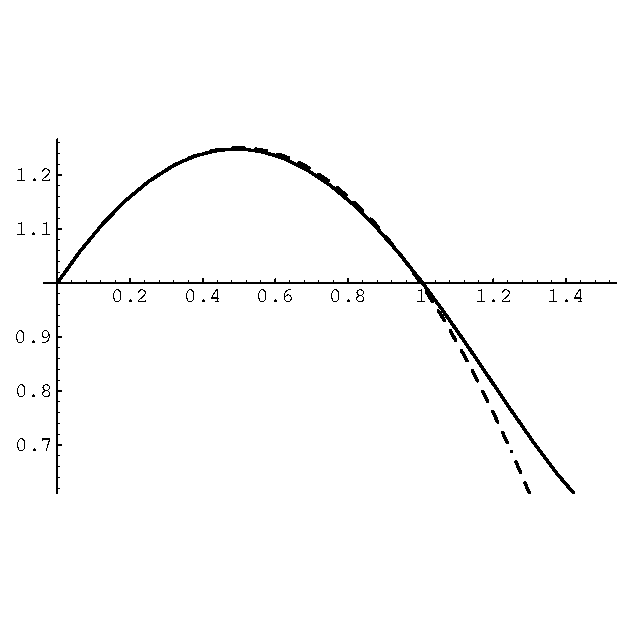
\includegraphics[width=0.4\textwidth]{ode/series/ndsftc}
    \end{center}
    \caption{Plot of the numerical solution and the first three terms in the
      Taylor series.}
    \label{ndsftc}
  \end{figure}
\end{Example}











The general recurrence relation for the $a_n$'s is useful if you only want to
calculate the first few terms in the Taylor expansion.  However,
for many problems substituting the Taylor series for the 
coefficient functions into the differential equation will enable you to 
find a simpler form of the solution.
We consider the following example to illustrate this point.





\begin{Example}
  Develop a series expansion of the solution to the initial value problem
  \[ w'' + \frac{1}{(z^2+1)} w = 0, \qquad w(0) = 1, \quad w'(0) = 0.\]

  \paragraph{Solution using the General Recurrence Relation.}
  The coefficient function has the Taylor expansion
  \[ \frac{1}{1+z^2} = \sum_{n=0}^\infty (-1)^n z^{2n}. \]
  From the initial condition we obtain $a_0 = 1$ and $a_1 = 0$.
  Thus we see that the solution is
  \[ w = \sum_{n=0}^\infty a_n z^n, \]
  where
  \[ a_{n+2} = -\frac{1}{(n+1)(n+2)} \sum_{m=0}^n a_m q_{n-m} \]
  and 
  \[ q_n =        \begin{cases}
    0 \quad &\mathrm{for odd}\ n \\
    (-1)^{(n/2)} \quad &\mathrm{for even}\ n.
  \end{cases}
  \]
  Although this formula is fine if you only want to calculate the first 
  few $a_n$'s, it is just a tad unwieldy to work with.  Let's see if we
  can get a better expression for the solution.

  \paragraph{Substitute the Taylor Series into the Differential Equation.}
  Substituting a Taylor series for $w$ yields
  \[ \frac{\dd^2}{\dd z^2} \sum_{n=0}^\infty a_n z^n + \frac{1}{(z^2 + 1)}
  \sum_{n=0}^\infty a_n z^n=0. \]
  Note that the algebra will be easier if we multiply by $z^2+1$.  The 
  polynomial $z^2+1$ has only two terms, but the Taylor series for
  $1/(z^2+1)$ has an infinite number of terms.
  \begin{gather*}
    (z^2 + 1)\frac{\dd^2}{\dd z^2} \sum_{n=0}^\infty a_n z^n + \sum_{n=0}^\infty a_n z^n=0\\
    \sum_{n=2}^\infty n(n-1)a_n z^n + \sum_{n=2}^\infty n(n-1)a_n z^{n-2}
    + \sum_{n=0}^\infty a_n z^n = 0 \\
    \sum_{n=0}^\infty n(n-1)a_n z^n
    + \sum_{n=0}^\infty (n+2)(n+1)a_{n+2} z^n
    + \sum_{n=0}^\infty a_n z^n = 0 \\
    \sum_{n=0}^\infty \Big[(n+2)(n+1)a_{n+2} + n(n-1)a_n + a_n \Big] z^n = 0
  \end{gather*}
  Equating powers of $z$ gives us the difference equation
  \[a_{n+2} = - \frac{n^2 - n + 1}{(n+2)(n+1)}a_n, \qquad \mathrm{for}\ n \geq 0.\]
  From the initial conditions we see that $a_0 = 1$ and $a_1 = 0$.  
  All of the odd terms in the series will be zero.  
  For the even terms, it is easier to reformulate the problem with 
  the change of variables 
  $b_n = a_{2n}$.  In terms of $b_n$ the difference equation is
  \[ b_{n+1} = - \frac{(2n)^2 - 2n + 1}{(2n+2)(2n+1)}b_{n}, \qquad b_0 = 1.\]
  This is a first order difference equation with the solution
  \[b_n = \prod_{j=0}^n \left(- \frac{4j^2 - 2j + 1}{(2j+2)(2j+1)}\right).\]
  Thus we have that
  \[a_n = 
  \begin{cases}
    \prod_{j=0}^{n/2} \left(- \frac{4j^2 - 2j + 1}{(2j+2)(2j+1)}\right)
    \quad &\mathrm{for even}\ n, \\
    0 & \mathrm{for odd}\  n.
  \end{cases}
  \]

  Note that the nearest singularities of $1/(z^2+1)$ in the complex plane are
  at $z = \pm i$.  Thus the radius of convergence must be at
  least $1$. 
  Applying the ratio test, the series converges for values of $|z|$ such that
  \begin{gather*}
    \lim_{n \to \infty} \left| \frac{a_{n+2} z^{n+2}}{a_n z^n}\right| < 1 \\
    \lim_{n \to \infty} \left| - \frac{n^2 - n + 1}{(n+2)(n+1)}\right| |z|^2
    < 1 \\
    |z|^2 < 1.
  \end{gather*}
  The radius of convergence is $1$.

  The first few terms in the Taylor expansion are
  \[ \boxed{ w = 1 - \frac{1}{2} z^2 + \frac{1}{8} z^4- \frac{13}{240}z^6 
    + \cdots.}\]

  In Figure~\ref{taylor_conv} the plot of the first two nonzero 
  terms is shown in a short
  dashed line, the plot of the first four nonzero terms is shown in a long dashed
  line, and the numerical solution is shown in a solid line.

  \begin{figure}[tb!]
    \begin{center} 
      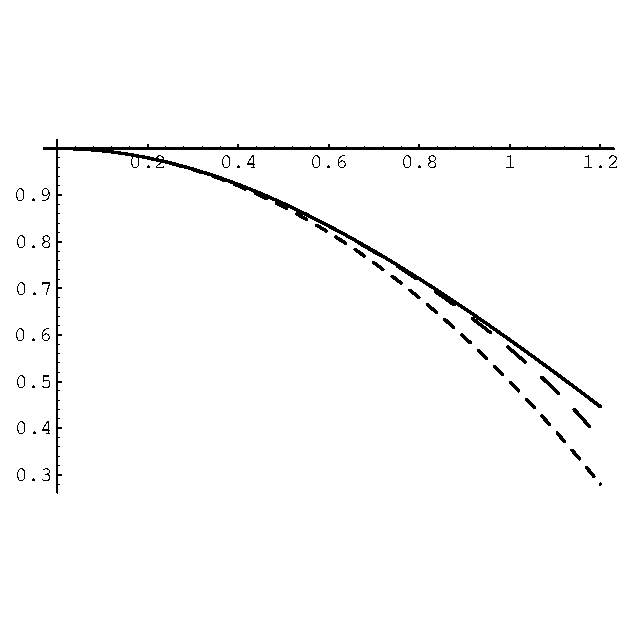
\includegraphics[width=0.4\textwidth]{ode/series/conv1}
    \end{center}
    \caption{Plot of the solution and approximations.}
    \label{taylor_conv}
  \end{figure}

\end{Example}











In general, if the coefficient functions are rational functions, that is
they are fractions of polynomials, multiplying the equations
by the quotient will reduce the algebra involved in finding the series
solution.




\begin{Example}
  If we were going to find the Taylor series expansion about $z=0$
  of the solution to
  \[ w'' + \frac{z}{1+z} w' + \frac{1}{1-z^2} w = 0,\]
  we would first want to multiply the equation by $1-z^2$ to obtain
  \[ (1-z^2) w'' + z (1-z) w'' + w = 0. \]
\end{Example}

























\begin{Example}
  Find the series expansions about $z=0$ of the fundamental set of solutions
  for
  \[ w'' +z^2 w = 0. \]
  Recall that the fundamental set of solutions $\{w_1, w_2\}$ satisfy
  \begin{alignat*}{2}
    w_1(0) &= 1 &\qquad w_2(0) &= 0 \\
    w_1'(0) &= 0 & \qquad w_2'(0) &= 1.
  \end{alignat*}
  Thus if
  \[ w_1 = \sum_{n=0}^\infty a_n z^n \qquad \mathrm{and} \qquad
  w_2 = \sum_{n=0}^\infty b_n z^n,\]
  then the coefficients must satisfy
  \[ a_0 = 1, \quad a_1 = 0, \qquad \mathrm{and} \qquad b_0=0, \quad b_1=1.\]

  Substituting the Taylor expansion $w = \sum_{n=0}^\infty c_n z^n$ into
  the differential equation,
  \begin{gather*}
    \sum_{n=2}^\infty n(n-1)c_n z^{n-2} + \sum_{n=0}^\infty c_n z^{n+2} = 0 \\
    \sum_{n=0}^\infty (n+2)(n+1) c_{n+2} z^n + \sum_{n=2}^\infty c_{n-2}z^n = 0 \\
    2c_2 + 6 c_3 z + \sum_{n=2}^\infty \Big[(n+2)(n+1)c_{n+2} + c_{n-2}\Big]z^n = 0
  \end{gather*}
  Equating coefficients of powers of $z$,
  \begin{alignat*}{2}
    &z^0: & \quad &c_2 = 0 \\
    &z^1: &\quad &c_3 = 0 \\
    &z^n: &\quad &(n+2)(n+1)c_{n+2} + c_{n-2} = 0, 
    \quad \mathrm{for}\ n \geq 2 \\
    &       &    &c_{n+4} = -\frac{c_n}{(n+4)(n+3)}
  \end{alignat*}

  For our first solution we have the difference equation
  \[ a_0 = 1,\ a_1 = 0,\ a_2 = 0,\ a_3 = 0, \qquad 
  a_{n+4} = -\frac{a_n}{(n+4)(n+3)}.\]
  For our second solution,
  \[ b_0 = 0,\ b_1 = 1,\ b_2 = 0,\ b_3 = 0, \qquad 
  b_{n+4} = -\frac{b_n}{(n+4)(n+3)}.\]
  The first few terms in the fundamental set of solutions are
  \[
  \boxed{
    w_1 = 1 - \frac{1}{12} z^4 + \frac{1}{672} z^8 - \cdots, \qquad 
    w_2 = z - \frac{1}{20} z^5 + \frac{1}{1440} z^9 - \cdots.
    }
  \]

  In Figure~\ref{w_one_two} the five term approximation is graphed
  in a coarse dashed line, the ten term approximation is graphed
  in a fine dashed line, and the numerical solution of $w_1$ is graphed in 
  a solid line.
  The same is done for $w_2$.

  \begin{figure}[tb!]
    \begin{center}
      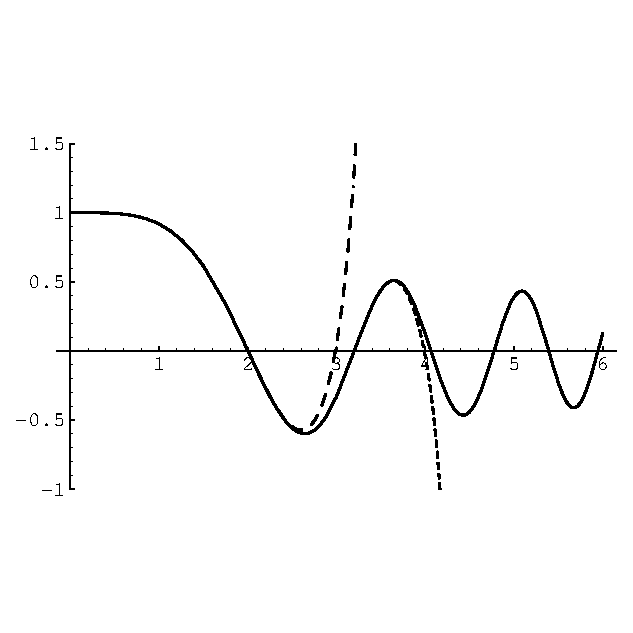
\includegraphics[width=0.4\textwidth]{ode/series/w_one}
      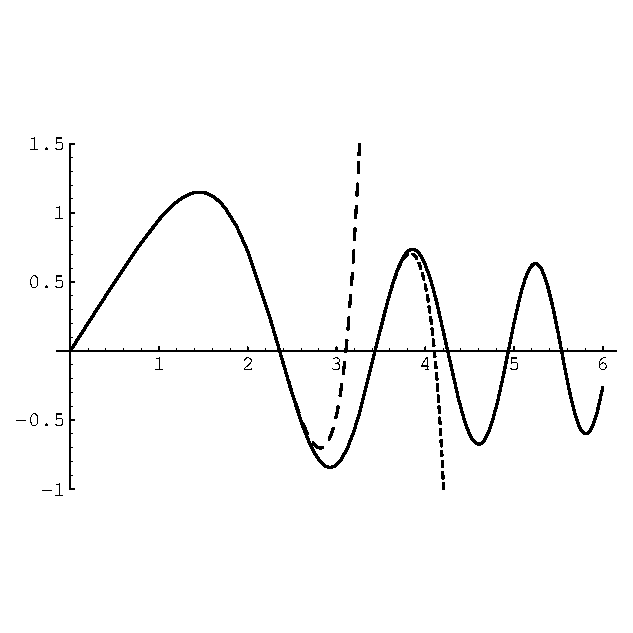
\includegraphics[width=0.4\textwidth]{ode/series/w_two}
    \end{center}
    \caption{The graph of the approximations and the numerical solution.}
    \label{w_one_two}
  \end{figure}


\end{Example}






\begin{Result}
  Consider the $n^{t h}$ order linear homogeneous equation
  \[ \frac{d^n w}{dz^n} + p_{n-1}(z) \frac{d^{n-1}w}{dz^{n-1}} + \cdots
  + p_1(z) \frac{\dd w}{\dd z} + p_0(z) w  = 0.\]
  If each of the coefficient functions $p_i(z)$ are analytic at $z=z_0$
  then $z_0$ is an ordinary point of the differential equation.
  The solution is analytic in some region containing $z_0$ and can
  be expanded in a Taylor series.  The radius of convergence of the
  series will be at least the distance to the nearest singularity of
  the coefficient functions in the complex plane.
\end{Result}
















%%===========================================================================
\section{Regular Singular Points of Second Order Equations}
Consider the differential equation
\[ w'' + \frac{p(z)}{z-z_0} w' + \frac{q(z)}{(z-z_0)^2} w = 0.\]
If $z=z_0$ is not an ordinary point but both $p(z)$ and $q(z)$ are 
analytic at $z=z_0$ then $z_0$ is a \textbf{regular singular point} of the 
differential equation.  The following equations have a regular singular
point at $z=0$.
\begin{itemize}
\item $w'' + \frac{1}{z} w' + z^2 w = 0$
\item $w'' + \frac{1}{\sin z} w' - w = 0$
\item $w'' - z w' + \frac{1}{z \sin z} w = 0$
\end{itemize}

Concerning regular singular points of second order linear equations there
is good news and bad news.

\paragraph{The Good News.} We will find that with the use of the Frobenius 
method we can always find series expansions
of two linearly independent solutions at a regular singular point.  
We will illustrate this theory with several examples.

\paragraph{The Bad News.} Instead of a tidy little theory like we have for 
ordinary points, the solutions can be of several different forms.
Also, for some of the problems the algebra can get pretty ugly.




\begin{Example}
  Consider the equation
  \[w'' + \frac{3(1+z)}{16z^2}w = 0.\]
  We wish to find series solutions about the point $z = 0$.  First we try
  a Taylor series $w = \sum_{n=0}^\infty a_n z^n$.
  Substituting this into the differential equation,
  \begin{gather*}
    z^2 \sum_{n=2}^\infty n(n-1)a_n z^{n-2} 
    + \frac{3}{16}(1+z) \sum_{n=0}^\infty a_n z^n = 0 \\
    \sum_{n=0}^\infty n(n-1)a_n z^n + \frac{3}{16} \sum_{n=0}^\infty a_n z^n
    + \frac{3}{16} \sum_{n=1}^\infty a_{n+1}z^n = 0.
  \end{gather*}
  Equating powers of $z$,
  \begin{alignat*}{2}
    &z^0: &\qquad &a_0 = 0 \\
    &z^n: &\qquad & \left[n(n-1) + \frac{3}{16}\right]a_n + \frac{3}{16} a_{n+1} 
    = 0 \\
    &       &       &a_{n+1} = \left[\frac{16}{3}n(n-1) + 1\right]a_n.
  \end{alignat*}
  This difference equation has the solution $a_n=0$ for all $n$.  Thus we have
  obtained only the trivial solution to the differential equation.  We must
  try an expansion of a more general form.  We recall that for regular singular
  points of first order equations we can always find a solution in the form
  of a Frobenius series $w = z^\alpha \sum_{n=0}^\infty a_n z^n$, $a_0\neq 0$.
  We substitute this series into the differential equation.
  \begin{gather*}
    z^2 \sum_{n=0}^\infty \big[\alpha(\alpha-1)+ 2 \alpha  n + n(n-1) \big] 
    a_n z^{n + \alpha - 2}
    + \frac{3}{16}(1+z)z^\alpha \sum_{n=0}^\infty a_n z^n = 0 \\
    \sum_{n=0}^\infty \big[\alpha(\alpha-1) + 2 n + n(n-1)\big]a_n z^n
    + \frac{3}{16} \sum_{n=0}^\infty a_n z^n
    + \frac{3}{16} \sum_{n=1}^\infty a_{n-1} z^n = 0 
  \end{gather*}
  Equating the $z^0$ term to zero yields the equation
  \[ \left(\alpha(\alpha-1) + \frac{3}{16}\right)a_0 = 0.\]
  Since we have assumed that $a_0\neq 0$, the polynomial in $\alpha$ must
  be zero.  The two roots of the polynomial are
  \[ \alpha_1 = \frac{1+\sqrt{1 - 3/4}}{2} = \frac{3}{4}, \qquad
  \alpha_2 = \frac{1-\sqrt{1 - 3/4}}{2} = \frac{1}{4}.\]
  Thus our two series solutions will be of the form
  \[ w_1 = z^{3/4}\sum_{n=0}^\infty a_n z^n, \qquad
  w_2 = z^{1/4}\sum_{n=0}^\infty b_n z^n.\]

  Substituting the first series into the differential equation,
  \begin{gather*}
    \sum_{n=0}^\infty \left[-\frac{3}{16} + 2n + n(n-1) + \frac{3}{16}\right]a_n z^n
    + \frac{3}{16} \sum_{n=1}^\infty a_{n-1} z^n = 0. 
  \end{gather*}
  Equating powers of $z$, we see that $a_0$ is arbitrary and
  \[ a_n = - \frac{3}{16n(n+1)} a_{n-1} \quad \mathrm{for}\ n \geq 1.\]
  This difference equation has the solution
  \begin{align*} 
    a_n &= a_0 \prod_{j=1}^n \left(-\frac{3}{16j(j+1)}\right) \\
    &= a_0 \left(-\frac{3}{16}\right)^n \prod_{j=1}^n \frac{1}{j(j+1)} \\
    &= a_0 \left(-\frac{3}{16}\right)^n \frac{1}{n!(n+1)!} 
    \quad \mathrm{for}\ n \geq 1.
  \end{align*}

  Substituting the second series into the differential equation,
  \begin{gather*}
    \sum_{n=0}^\infty \left[-\frac{3}{16} + 2n + n(n-1) + \frac{3}{16}\right]b_n z^n
    + \frac{3}{16} \sum_{n=1}^\infty b_{n-1} z^n = 0. 
  \end{gather*}
  We see that the difference equation for $b_n$ is the same as the 
  equation for $a_n$.  Thus we can write the general solution to the 
  differential equation as
  \[w = c_1 z^{3/4} \left(1 + \sum_{n=1}^\infty 
    \left(-\frac{3}{16}\right)^n \frac{1}{n!(n+1)!} z^n \right)
  + c_2 z^{1/4} \left(1 + \sum_{n=1}^\infty 
    \left(-\frac{3}{16}\right)^n \frac{1}{n!(n+1)!} z^n \right) \]
  \[ \boxed{ \left(c_1 z^{3/4} + c_2 z^{1/4}\right) \left(1 + \sum_{n=1}^\infty 
      \left(-\frac{3}{16}\right)^n \frac{1}{n!(n+1)!} z^n \right).}\]
\end{Example}











\subsection{Indicial Equation}
\index{indicial equation}
Now let's consider the general equation for a regular singular point at
$z = 0$
\[ w'' + \frac{p(z)}{z} w' + \frac{q(z)}{z^2} w = 0.\]
Since $p(z)$ and $q(z)$ are analytic at $z=0$ we can expand them in
Taylor series.
\[ p(z) = \sum_{n=0}^\infty p_n z^n, 
\qquad q(z) = \sum_{n=0}^\infty q_n z^n \]
Substituting a Frobenius series $w = z^\alpha \sum_{n=0}^\infty a_n z^n,\ 
a_0 \neq 0$ and the Taylor series for $p(z)$ and $q(z)$ into the differential
equation yields
\[\sum_{n=0}^\infty \Big[(\alpha+n)(\alpha+n-1)\Big]a_n z^n
+ \left(\sum_{n=0}^\infty p_n z^n\right)
\left(\sum_{n=0}^\infty (\alpha+n) a_n z^n\right)
+ \left(\sum_{n=0}^\infty q_n z^n\right)\left(\sum_{n=0}^\infty a_n z^n\right) = 0\]
\begin{align*}
  &\sum_{n=0}^\infty \Big[(\alpha+n)^2 - (\alpha+n) + p_0(\alpha+n)+q_0 \Big]a_n z^n \\
  &\qquad \qquad \qquad + \left(\sum_{n=1}^\infty p_n z^n\right)
  \left(\sum_{n=0}^\infty (\alpha+n) a_n z^n\right)
  + \left(\sum_{n=1}^\infty q_n z^n\right)\left(\sum_{n=0}^\infty a_n z^n\right) = 0
\end{align*}
\[\sum_{n=0}^\infty \Big[(\alpha+n)^2 + (p_0-1)(\alpha_n) + q_0 \Big]a_n z^n
+ \sum_{n=1}^\infty \left( \sum_{j=0}^{n-1} (\alpha+j) a_j p_{n-j}
\right) z^n
+ \sum_{n=1}^\infty \left( \sum_{j=0}^{n-1} a_j q_{n-j} \right) z^n = 0\]


Equating powers of $z$,
\begin{alignat*}{2}
  &z^0: &\quad    &\Big[\alpha^2 + (p_0-1)\alpha + q_0\Big]a_0 = 0 \\
  &z^n: &\quad    &\Big[(\alpha+n)^2 + (p_0-1)(\alpha+n) + q_0\Big]a_n
  = -\sum_{j=0}^{n-1}\Big[(\alpha+j)p_{n-j} + q_{n-j}\Big]a_j.
\end{alignat*}
Let
\[ I(\alpha) = \alpha^2 + (p_0-1)\alpha + q_0 = 0.\]
This is known as the \textbf{indicial equation}.  
The indicial equation gives us the 
form of the solutions.  
The equation for $a_0$ is $I(\alpha)a_0 = 0$.  Since we assumed that $a_0$
is nonzero, $I(\alpha) = 0$.  Let the two roots of $I(\alpha)$ be 
$\alpha_1$ and $\alpha_2$ where $\Re(\alpha_1) \geq \Re(\alpha_2)$.

Rewriting the difference equation for $a_n(\alpha)$,
\begin{equation} \label{diff-a_n}
  I(\alpha+n)a_n(\alpha) 
  = - \sum_{j=0}^{n-1}\Big[(\alpha+j)p_{n-j} + q_{n-j}\Big]a_j(\alpha)
  \quad \mathrm{for}\ n \geq 1.
\end{equation}

If the roots are distinct and do not differ by an integer
then we can use Equation~\ref{diff-a_n} to solve for $a_n(\alpha_1)$
and $a_n(\alpha_2)$, which will give us the two solutions
\[ w_1 = z^{\alpha_1} \sum_{n=0}^\infty a_n(\alpha_1)z^n, \quad \mathrm{and} \quad
w_2 = z^{\alpha_2} \sum_{n=0}^\infty a_n(\alpha_2)z^n.\]

If the roots are not distinct, $\alpha_1 = \alpha_2$, we will only have one
solution and will have to generate another.  If the roots differ by an
integer, $\alpha_1 - \alpha_2 = N$, there is one solution corresponding
to $\alpha_1$, but when we try to solve Equation~\ref{diff-a_n} for 
$a_n(\alpha_2)$, we will encounter the equation
\[ I(\alpha_2 + N)a_N(\alpha_2) = I(\alpha_1)a_N(\alpha_2) 
= 0 \cdot a_N(\alpha_2)
= -\sum_{j=0}^{N-1}\Big[(\alpha+n)p_{n-j} + q_{n-j}\Big]a_j(\alpha_2).\]
If the right side of the equation is nonzero, then $a_N(\alpha_2)$ is
undefined.  On the other hand, 
if the right side is zero then $a_N(\alpha_2)$ is arbitrary.
The rest of this section is devoted to considering the cases 
$\alpha_1 = \alpha_2$ and $\alpha_1 - \alpha_2 = N$.

























\subsection{The Case: Double Root}
Consider a second order equation $L[w] = 0$ with a regular singular point
at $z = 0$.  Suppose the indicial equation has a double root.
\[ I(\alpha) = (\alpha-\alpha_1)^2 = 0\]
One solution has the form
\[ w_1 = z^{\alpha_1} \sum_{n=0}^\infty a_n z^n.\]
In order to find the second solution, we will differentiate with respect to the 
parameter, $\alpha$.  Let $a_n(\alpha)$ satisfy Equation~\ref{diff-a_n}
Substituting the Frobenius expansion into the differential equation,
\[ L\left[z^\alpha \sum_{n=0}^\infty a_n(\alpha) z^n\right] = 0.\]
Setting $\alpha=\alpha_1$ will make the left hand side of the equation zero.
Differentiating this equation with respect to $\alpha$,
\[ \frac{\partial}{\partial \alpha}L\left[z^\alpha \sum_{n=0}^\infty a_n(\alpha) z^n\right] 
= 0.\]
Interchanging the order of differentiation,
\[ L\left[ \log z\,z^\alpha \sum_{n=0}^\infty a_n(\alpha) z^n
  + z^\alpha \sum_{n=0}^\infty \frac{\dd a_n(\alpha)}{\dd \alpha} z^n \right]
= 0.\]
Since setting $\alpha = \alpha_1$ will make the left hand side of this 
equation zero, the second linearly independent solution is
\[ w_2 = \log z\, z^{\alpha_1} \sum_{n=0}^\infty a_n(\alpha_1) z^n
+ z^{\alpha_1} \sum_{n=0}^\infty \frac{\dd a_n(\alpha)}{\dd \alpha} 
\Bigg|_{\alpha=\alpha_1} z^n  \]
\[ \boxed{ w_2 = w_1 \log z
  + z^{\alpha_1} \sum_{n=0}^\infty a_n'(\alpha_1)
  z^n .} \]













\begin{Example}
  Consider the differential equation
  \[ w'' + \frac{1+z}{4z^2} w = 0.\]
  There is a regular singular point at $z = 0$.  The indicial equation is
  \[ \alpha(\alpha-1) + \frac{1}{4} = \left(\alpha-\frac{1}{2}\right)^2 = 0.\]
  One solution will have the form
  \[ w_1 = z^{1/2} \sum_{n=0}^\infty a_n z^n , \quad a_0 \neq 0.\]

  Substituting the Frobenius expansion
  \[z^\alpha \sum_{n=0}^\infty a_n(\alpha) z^n\]
  into the differential equation yields
  \begin{gather*}
    z^2 w'' + \frac{1}{4}(1+z) w = 0 \\
    \sum_{n=0}^\infty \big[\alpha(\alpha-1) + 2 \alpha n + n(n-1)  \big]
    a_n(\alpha) z^{n+\alpha}
    + \frac{1}{4} \sum_{n=0}^\infty a_n(\alpha) z^{n+\alpha}
    + \frac{1}{4} \sum_{n=0}^\infty a_n(\alpha) z^{n+\alpha+1} = 0. \\
    \intertext{Divide by $z^\alpha$ and adjust the summation indices.}
    \sum_{n=0}^\infty \left[\alpha(\alpha-1) + 2 \alpha n + n(n-1)  \right]
    a_n(\alpha) z^n
    + \frac{1}{4} \sum_{n=0}^\infty a_n(\alpha) z^n
    + \frac{1}{4} \sum_{n=1}^\infty a_{n-1}(\alpha) z^n = 0 \\
    \left[\alpha(\alpha-1)a_0 + \frac{1}{4}\right]a_0
    + \sum_{n=1}^\infty \left(\left[\alpha(\alpha-1) + 2 n + n(n-1) 
        + \frac{1}{4}\right]a_n(\alpha) + \frac{1}{4} a_{n-1}(\alpha)
    \right) z^n=0
  \end{gather*}
  Equating the coefficient of $z^0$ to zero yields $I(\alpha) a_0 = 0$.
  Equating the coefficients of $z^n$ to zero yields the difference equation
  \begin{gather*}
    \left[\alpha(\alpha-1) + 2 n + n(n-1) 
      + \frac{1}{4}\right]a_n(\alpha) + \frac{1}{4} a_{n-1}(\alpha) = 0 \\
    a_n(\alpha) = - \left(\frac{n(n+1)}{4} + \frac{\alpha(\alpha-1)}{4} 
      + \frac{1}{16} \right)a_{n-1}(\alpha).
  \end{gather*}
  The first few $a_n$'s are
  \[ a_0,\quad -\left(\alpha(\alpha-1) + \frac{9}{16} \right)a_0, \quad
  \left(\alpha(\alpha-1) + \frac{25}{16} \right)
  \left(\alpha(\alpha-1) + \frac{9}{16} \right)a_0,\ldots \]
  Setting $\alpha=1/2$, the coefficients for the first solution are
  \[a_0,\quad  -\frac{5}{16} a_0,\quad \frac{105}{16}a_0,\quad \ldots\]

  The second solution has the form
  \[ w_2 = w_1 \log z 
  + z^{1/2} \sum_{n=0}^\infty a_n'(1/2) z^n.\]
  Differentiating the $a_n(\alpha)$, 
  \[ \frac{\dd a_0}{\dd \alpha} = 0, 
  \quad  \frac{\dd a_1(\alpha)}{\dd \alpha} = -(2\alpha - 1)a_0,\quad  
  \frac{\dd a_2(\alpha)}{\dd \alpha} = 
  (2\alpha-1)\left[\left(\alpha(\alpha-1) + \frac{9}{16} \right)+ 
    \left(\alpha(\alpha-1) + \frac{25}{16} \right)
  \right]a_0,\quad \ldots\]
  Setting $\alpha = 1/2$ in this equation yields
  \[ a_0' = 0,\quad a_1'(1/2) = 0,\quad a_2'(1/2) = 0,\quad \ldots\]
  Thus the second solution is
  \[ w_2 = w_1 \log z .\]
  The first few terms in the general solution are
  \[ \boxed{(c_1 + c_2 \log z)\left(1 - \frac{5}{16}z + \frac{105}{16}z^2 
      - \cdots \right).}\]
\end{Example}














\subsection{The Case: Roots Differ by an Integer}
Consider the case in which the roots of the indicial equation $\alpha_1$
and $\alpha_2$ differ by an integer. ($\alpha_1 - \alpha_2 = N$) 
Recall the equation that determines $a_n(\alpha)$ 
\[ I(\alpha+n)a_n = \Big[(\alpha+n)^2 + (p_0-1)(\alpha+n)+q_0\Big]a_n 
= - \sum_{j=0}^{n-1} \Big[(\alpha+j)p_{n-j} + q_{n-j}\Big]a_j.\]
When $\alpha = \alpha_2$ the equation for $a_N$ is
\[ I(\alpha_2 + N) a_N(\alpha_2) = 0 \cdot a_N(\alpha_2)  
= - \sum_{j=0}^{N-1} \Big[(\alpha+j)p_{N-j} + q_{N-j}\Big]a_j.\]
If the right hand side of this equation is zero, then $a_N$ is arbitrary.
There will
be two solutions of the Frobenius form.
\[ w_1 = z^{\alpha_1} \sum_{n=0}^\infty a_n(\alpha_1) z^n \quad \mathrm{and} \quad
w_2 = z^{\alpha_2} \sum_{n=0}^\infty a_n(\alpha_2) z^n.\]
If the right hand side of the equation is nonzero
then $a_N(\alpha_2)$ will be undefined.
We will have to generate the second solution.  Let
\[ w(z,\alpha) = z^\alpha \sum_{n=0}^\infty a_n(\alpha) z^n,\]
where $a_n(\alpha)$ satisfies the recurrence formula.
Substituting this series into the differential equation yields
\[ L[w(z,\alpha)] = 0.\]
We will multiply by $(\alpha-\alpha_2)$, 
differentiate this equation with respect to $\alpha$ and then set
$\alpha = \alpha_2$.  This will generate a linearly independent solution.
\begin{align*}
  \frac{\partial}{\partial \alpha} L[(\alpha-\alpha_2) w(z, \alpha)]
  &= L\left[ \frac{\partial}{\partial \alpha} (\alpha-\alpha_2)w(z,\alpha) \right] \\
  &= L\left[ \frac{\partial}{\partial \alpha} (\alpha-\alpha_2)
    z^\alpha \sum_{n=0}^\infty a_n(\alpha) z^n \right] \\
  &= L\left[ \log z\ z^\alpha \sum_{n=0}^\infty (\alpha-\alpha_2)a_n(\alpha)z^n
    +z^\alpha \sum_{n=0}^\infty \frac{\dd}{\dd \alpha} [(\alpha-\alpha_2)
    a_n(\alpha)] z^n \right]
\end{align*}
Setting $\alpha = \alpha_2$ with make this expression zero, thus
\[ \log z\ z^\alpha \sum_{n=0}^\infty \lim_{\alpha \to \alpha_2} 
\left\{ (\alpha-\alpha_2)a_n(\alpha) \right\} z^n
+z^{\alpha_2} \sum_{n=0}^\infty \lim_{\alpha \to \alpha_2} \left\{
  \frac{\dd}{\dd \alpha} [(\alpha-\alpha_2)a_n(\alpha)] \right\} z^n \]
is a solution.
Now let's look at the first term in this solution
\[ \log z\ z^\alpha \sum_{n=0}^\infty \lim_{\alpha \to \alpha_2}
\left\{ (\alpha-\alpha_2)a_n(\alpha) \right\} z^n. \]
The first $N$ terms in the sum will be zero.   
That is because $a_0, \ldots, a_{N-1}$ are finite, so multiplying by 
$(\alpha-\alpha_2)$ and taking the limit as $\alpha \to \alpha_2$ will make
the coefficients vanish.
The equation for $a_N(\alpha)$ is
\[ I(\alpha + N) a_N(\alpha) 
= - \sum_{j=0}^{N-1} \Big[(\alpha+j)p_{N-j} + q_{N-j}\Big]a_j(\alpha). \]
Thus the coefficient of the $N^{t h}$ term is
\begin{align*}
  \lim_{\alpha \to \alpha_2}(\alpha-\alpha_2)a_N(\alpha)
  &= -\lim_{\alpha \to \alpha_2} \left[ \frac{(\alpha-\alpha_2)}
    {I(\alpha+N)}\sum_{j=0}^{N-1} 
    \Big[(\alpha+j)p_{N-j} + q_{N-j}\Big]a_j(\alpha) \right]\\
  &= -\lim_{\alpha \to \alpha_2} \left[ \frac{(\alpha-\alpha_2)}
    {(\alpha + N - \alpha_1)(\alpha+N-\alpha_2)}\sum_{j=0}^{N-1} 
    \Big[(\alpha+j)p_{N-j} + q_{N-j}\Big]a_j(\alpha) \right]\\
  \intertext{Since $\alpha_1 = \alpha_2 + N$, $\lim_{\alpha \to \alpha_2} 
    \frac{\alpha-\alpha_2}{\alpha+N-\alpha_1} = 1$.}
  &= -\frac{1}{(\alpha_1 - \alpha_2)}\sum_{j=0}^{N-1} 
  \Big[(\alpha_2+j)p_{N-j} + q_{N-j}\Big]a_j(\alpha_2) .
\end{align*}
Using this you can show that the first term in the solution can be written
\[ d_{-1} \log z\ w_1, \]
where $d_{-1}$ is a constant.
Thus the second linearly independent solution is
\[ \boxed{ w_2 = d_{-1} \log z\ w_1 + 
  z^{\alpha_2} \sum_{n=0}^\infty d_n z^n, } \]
where
\[ d_{-1} = - \frac{1}{a_0} 
\frac{1}{(\alpha_1 - \alpha_2)}\sum_{j=0}^{N-1}
\Big[(\alpha_2+j)p_{N-j} + q_{N-j}\Big]a_j(\alpha_2) \]
and
\[ d_n = \lim_{\alpha \to \alpha_2} \left\{
  \frac{\dd}{\dd \alpha} \Big[(\alpha-\alpha_2)a_n(\alpha)\Big] \right\} 
\quad \mathrm{for}\ n \geq 0. \]













\begin{Example}
  Consider the differential equation
  \[ w'' + \left(1 - \frac{2}{z} \right) w' + \frac{2}{z^2} w = 0. \]
  The point $z = 0$ is a regular singular point.  In order to find series
  expansions of the solutions, we first calculate the indicial equation.
  We can write the coefficient functions in the form
  \[ \frac{p(z)}{z} = \frac{1}{z}(-2 + z), \quad \mathrm{and} \quad
  \frac{q(z)}{z^2} = \frac{1}{z^2}(2). \]
  Thus the indicial equation is
  \begin{gather*}
    \alpha^2 + (-2-1)\alpha + 2 = 0 \\
    (\alpha-1)(\alpha-2) = 0.
  \end{gather*}

  \paragraph{The First Solution.}
  The first solution will have the Frobenius form
  \[ w_1 = z^2 \sum_{n=0}^\infty a_n(\alpha_1) z^n. \]
  Substituting a Frobenius series into the differential equation,
  \begin{gather*}
    z^2 w'' + (z^2 - 2z) w' + 2 w = 0 \\
    \sum_{n=0}^\infty (n + \alpha)(n + \alpha-1) z^{n+\alpha}
    + (z^2-2z) \sum_{n=0}^\infty (n+\alpha)z^{n+\alpha-1}
    + 2 \sum_{n=0}^\infty a_n z^n = 0 \\
    [\alpha^2 - 3 \alpha + 2]a_0 + \sum_{n=1}^\infty \Big[(n+\alpha)(n+\alpha-1)a_n 
    + (n + \alpha-1)a_{n-1}
    -2 (n+\alpha)a_n + 2a_n\Big] z^n = 0.
  \end{gather*}
  Equating powers of $z$,
  \begin{gather*}
    \Big[(n+\alpha)(n+\alpha-1)  -2 (n+\alpha) + 2\Big] a_n = - (n + \alpha-1)a_{n-1} \\
    a_n = - \frac{a_{n-1}}{n+\alpha-2} . 
  \end{gather*}

  Setting $\alpha = \alpha_1 = 2$, the recurrence relation becomes
  \begin{align*}
    a_n(\alpha_1) &= - \frac{a_{n-1}(\alpha_1)}{n} \\
    &= a_0 \frac{(-1)^n}{n!}. 
  \end{align*}
  The first solution is
  \[ \boxed{ w_1 = a_0 \sum_{n=0}^\infty \frac{(-1)^n}{n!} z^n 
    = a_0 \e^{-z}.} \]

  \paragraph{The Second Solution.}
  The equation for $a_1(\alpha_2)$ is
  \[ 0 \cdot a_1(\alpha_2) = 2 a_0. \]
  Since the right hand side of this equation is not 
  zero, the second solution will
  have the form
  \[ w_2 = d_{-1} \log z\ w_1 + 
  z^{\alpha_2} \sum_{n=0}^\infty \lim_{\alpha \to \alpha_2} \left\{
    \frac{\dd}{\dd \alpha} [(\alpha-\alpha_2)a_n(\alpha)] \right\}z^n \]

  First we will calculate $d_{-1}$ as we defined it previously.
  \[ d_{-1} = - \frac{1}{a_0} \frac{1}{2-1} a_0 = -1. \]
  The expression for $a_n(\alpha)$ is
  \[ a_n(\alpha) = \frac{(-1)^n a_0}{(\alpha+n-2)(\alpha+n-1) 
    \cdots(\alpha-1)}. \]
  The first few $a_n(\alpha)$ are
  \begin{align*}
    a_1(\alpha) &= - \frac{a_0}{\alpha-1} \\
    a_2(\alpha) &= \frac{a_0}{\alpha(\alpha-1)} \\
    a_3(\alpha) &= -\frac{a_0}{(\alpha+1)\alpha(\alpha-1)}.
  \end{align*}
  We would like to calculate
  \[ d_n = \lim_{\alpha \to 1} \left\{
    \frac{\dd}{\dd \alpha} \Big[(\alpha-1)a_n(\alpha)\Big] \right\}. \]
  The first few $d_n$ are
  \begin{align*}
    d_0     &= \lim_{\alpha \to 1} \left\{
      \frac{\dd}{\dd \alpha} \Big[(\alpha-1) a_0\Big] \right\} \\
    &= a_0 \\
    d_1     &= \lim_{\alpha \to 1} \left\{
      \frac{\dd}{\dd \alpha} \left[(\alpha-1)
        \left( - \frac{a_0}{\alpha-1} \right)\right] \right\} \\
    &= \lim_{\alpha \to 1} \left\{
      \frac{\dd}{\dd \alpha} \Big[-a_0\Big] \right\} \\
    &= 0 \\
    d_2     &= \lim_{\alpha \to 1} \left\{
      \frac{\dd}{\dd \alpha} \left[(\alpha-1)
        \left( \frac{a_0}{\alpha(\alpha-1)} \right)\right] \right\} \\
    &= \lim_{\alpha \to 1} \left\{
      \frac{\dd}{\dd \alpha} \left[\frac{a_0}{\alpha}\right]\right\} \\
    &= -a_0 \\
    d_3     &= \lim_{\alpha \to 1} \left\{
      \frac{\dd}{\dd \alpha} \left[(\alpha-1)
        \left( -\frac{a_0}{(\alpha+1)\alpha(\alpha-1)}
        \right)\right] \right\} \\
    &= \lim_{\alpha \to 1} \left\{
      \frac{\dd}{\dd \alpha} \left[-\frac{a_0}{(\alpha+1)\alpha} \right] \right\} \\
    &= \frac{3}{4}a_0.
  \end{align*}
  It will take a little work to find the general
  expression for $d_n$.  We will need the
  following relations.
  \[ \Gamma(n) = (n-1)!, \quad \Gamma'(z) = \Gamma(z) \psi(z), \quad
  \psi(n) = - \gamma + \sum_{k=1}^{n-1} \frac{1}{k}. \]
  See the chapter on the Gamma function for explanations of these equations.
  \begin{align*}
    d_n     &= \lim_{\alpha \to 1} \left\{
      \frac{\dd}{\dd \alpha} \left[(\alpha-1)
        \frac{(-1)^n a_0 }{(\alpha+n-2)(\alpha+n-1)\cdots(\alpha-1) }\right] 
    \right\} \\
    &= \lim_{\alpha \to 1} \left\{
      \frac{\dd}{\dd \alpha} \left[\frac{(-1)^n a_0 }{(\alpha+n-2)(\alpha+n-1)
          \cdots(\alpha)}\right]\right\} \\
    &= \lim_{\alpha \to 1} \left\{
      \frac{\dd}{\dd \alpha} \left[\frac{(-1)^n a_0 \Gamma(\alpha)}
        {\Gamma(\alpha+n-1)} \right] \right\} \\
    &= (-1)^n a_0 \lim_{\alpha \to 1} \left\{ \frac{\Gamma(\alpha)
        \psi(\alpha)}{\Gamma(\alpha+n-1)} - \frac{\Gamma(\alpha)
        \psi(\alpha+n-1)}{\Gamma(\alpha+n-1)} \right\} \\
    &= (-1)^n a_0 \lim_{\alpha \to 1} \left\{ \frac{\Gamma(\alpha)
        [\psi(\alpha)-\psi(\alpha+n-1)]}{\Gamma(\alpha+n-1)} \right\} \\
    &= (-1)^n a_0 \frac{\psi(1) - \psi(n)}{(n-1)!} \\
    &= \frac{(-1)^{n+1} a_0}{(n-1)!} \sum_{k=0}^{n-1} \frac{1}{k}
  \end{align*}
  Thus the second solution is
  \[ \boxed{ w_2 = -\log z\ w_1 + z \sum_{n=0}^\infty \left( \frac{(-1)^{n+1} a_0}
      {(n-1)!} \sum_{k=0}^{n-1} \frac{1}{k}\right) z^n.} \]
  The general solution is
  \[ \boxed{ w = c_1 \e^{-z} - c_2 \log z\ \e^{-z} + c_2 
    z \sum_{n=0}^\infty \left( \frac{(-1)^{n+1} }
      {(n-1)!} \sum_{k=0}^{n-1} \frac{1}{k}\right) z^n. } \]
\end{Example}


We see that even in problems that are chosen for their simplicity, the algebra
involved in the Frobenius method can be pretty involved.







\begin{Example}
  Consider a series expansion about the origin of the equation
  \[ w'' + \frac{1-z}{z} w' - \frac{1}{z^2} w = 0. \]

  The indicial equation is
  \begin{gather*}
    \alpha^2 -1 = 0 \\
    \alpha = \pm 1.
  \end{gather*}

  Substituting a Frobenius series into the differential equation,
  \begin{gather*}
    z^2 \sum_{n=0}^\infty (n+\alpha)(n+\alpha-1) a_n z^{n-2} + (z-z^2)\sum_{n=0}^\infty (n+\alpha)
    a_n z^{n-1} - \sum_{n=0}^\infty a_n z^n = 0 \\
    \sum_{n=0}^\infty (n+\alpha)(n+\alpha-1) a_n z^n + \sum_{n=0}^\infty (n+\alpha)a_n z^n
    - \sum_{n=1}^\infty (n+\alpha-1)a_{n-1}z^n - \sum_{n=0}^\infty a_n z^n = 0 \\
    \Big[\alpha(\alpha-1) + \alpha - 1\Big] a_0 
    + \sum_{n=1}^\infty \Big[n+\alpha)(n+\alpha-1) a_n
    + (n+\alpha-1) a_n - (n+\alpha-1)a_{n-1}\Big] z^n = 0.
  \end{gather*}
  Equating powers of $z$ to zero,
  \[ a_n(\alpha) = \frac{a_{n-1}(\alpha)}{n+\alpha+1} . \]

  We know that the first solution has the form
  \[ w_1 = z \sum_{n=0}^\infty a_n z^n. \]
  Setting $\alpha = 1$ in the reccurence formula,
  \[ a_n = \frac{a_{n-1}}{n+2} = \frac{2 a_0}{(n+2)!}. \]
  Thus the first solution is
  \begin{align*}
    w_1     &= z \sum_{n=0}^\infty \frac{2 a_0}{(n+2)!} z^n \\
    &= 2 a_0 \frac{1}{z} \sum_{n=0}^\infty \frac{z^{n+2}}{(n+2)!} \\
    &= \frac{2 a_0}{z} \left( \sum_{n=0}^\infty \frac{z^n}{n!} - 1 - z \right) \\
    &= \frac{2 a_0}{z} (\e^z - 1 - z).
  \end{align*}

  Now to find the second solution.  Setting $\alpha = -1$ in the reccurence 
  formula,
  \[ a_n = \frac{a_{n-1}}{n} = \frac{a_0}{n!}. \]
  We see that in this case there is no trouble in defining $a_2(\alpha_2)$.
  The second solution is
  \[ w_2 = \frac{a_0}{z} \sum_{n=0}^\infty \frac{z^n}{n!} = \frac{a_0}{z} \e^z. \]

  Thus we see that the general solution is
  \[ w = \frac{c_1}{z} (\e^z - 1 - z) + \frac{c_2}{z} \e^z \]
  \[ \boxed{ w = \frac{d_1}{z} \e^z + d_2 \left(1+\frac{1}{z} \right). } \]
\end{Example}




































%%===========================================================================
\section{Irregular Singular Points}
\index{irregular singular points}

If a point $z_0$ of a differential equation is not ordinary or regular 
singular, then it is an \textbf{irregular singular point}.
At least one of the solutions at an irregular singular point will not be of
the Frobenius form.  We will examine how to obtain series expansions about
an irregular singular point in the chapter on asymptotic expansions.













%%===========================================================================
\section{The Point at Infinity}
\index{point at infinity!differential equations}

If we want to determine the behavior of a function $f(z)$ at infinity,
we can make the transformation $\zeta = 1 / z$ and examine the point $\zeta = 0$.


\begin{Example}
  Consider the behavior of $f(z) = \sin z$ at infinity.
  This is the same as considering the point $\zeta = 0$ of $\sin(1/\zeta)$, which
  has the series expansion
  \[ 
  \sin \left( \frac{1}{\zeta} \right)
  = \sum_{n=0}^\infty \frac{(-1)^n}{(2 n + 1)! \zeta^{2n+1}}. 
  \]
  Thus we see that the point $\zeta = 0$ is an essential singularity of 
  $\sin(1/\zeta)$.  Hence $\sin z$ has an essential singularity at $z = \infty$.
\end{Example}







\begin{Example}
  Consider the behavior at infinity of $z \e^{1/z}$.  We make the transformation
  $\zeta = 1/z$.
  \[ 
  \frac{1}{\zeta} \e^\zeta = \frac{1}{\zeta} \sum_{n=0}^\infty \frac{\zeta^n}{n!}
  \]
  Thus $z \e^{1/z}$ has a pole of order $1$ at infinity.
\end{Example}






In order to classify the point at infinity of a differential equation
in $w(z)$, we apply the transformation $\zeta = 1/z$, $u(\zeta) = w(z)$.
We write the derivatives with respect to $z$ in terms of $\zeta$.
\begin{align*}
  z &= \frac{1}{\zeta} 
  \\
  \dd z &= - \frac{1}{\zeta^2} \dd \zeta 
  \\
  \frac{\dd}{\dd z} &= - \zeta^2 \frac{\dd}{\dd \zeta}
\end{align*}
\begin{align*}
  \frac{\dd^2}{\dd z^2} &= -\zeta^2 \frac{\dd}{\dd \zeta} \left( - \zeta^2 \frac{\dd}{\dd \zeta} 
  \right) 
  \\
  &= \zeta^4 \frac{\dd^2}{\dd \zeta^2} + 2 \zeta^3 \frac{\dd}{\dd \zeta}
\end{align*}
Now we apply the transformation to the differential equation.
\begin{gather*}
  w'' + p(z) w' + q(z) w = 0
  \\
  \zeta^4 u'' + 2 \zeta^3 u' + p(1/\zeta) (-\zeta^2) u' + q(1/\zeta) u = 0 
  \\
  u'' + \left( \frac{2}{\zeta} - \frac{p(1/\zeta)}{\zeta^2} \right) u'
  + \frac{q(1/\zeta)}{\zeta^4} u = 0
\end{gather*}





\begin{Example}
  Classify the singular points of the differential equation
  \[ 
  w'' + \frac{1}{z} w' + 2 w = 0. 
  \]

  There is a regular singular point at $z = 0$.  To examine the point 
  at infinity
  we make the transformation $\zeta = 1/z$, $u(\zeta) = w(z)$.
  \begin{gather*}
    u'' + \left( \frac{2}{\zeta} - \frac{1}{\zeta} \right) u' + \frac{2}{\zeta^4} u = 0 
    \\
    u'' + \frac{1}{\zeta}  u' + \frac{2}{\zeta^4} u = 0
  \end{gather*}
  Thus we see that the differential equation for $w(z)$ has an irregular 
  singular point at infinity.
\end{Example}






























\raggedbottom
%%===========================================================================
\exercises{
\pagebreak
\flushbottom
\section{Exercises}






%% Hermite equation
\begin{Exercise}[mathematica/ode/series/series.nb]
  \label{exercise hermite eqn}
  $f(x)$ satisfies the Hermite equation
  \[
  \frac{\dd^2 f}{\dd x^2} - 2 x \frac{\dd f}{\dd x} + 2 \lambda f = 0.
  \]
  Construct two linearly independent solutions of the equation as Taylor
  series about $x = 0$.  For what values of $x$ do the series converge?

  Show that for certain values of $\lambda$, called eigenvalues,
  one of the solutions is a polynomial, called an eigenfunction.
  Calculate the first four eigenfunctions $H_0(x)$, $H_1(x)$, $H_2(x)$,
  $H_3(x)$, ordered by degree.

  \hintsolution{hermite eqn}
\end{Exercise}





%% Legendre equation
\begin{Exercise}
  \label{exercise legendre eqn}
  Consider the Legendre equation
  \[
  (1-x^2) y'' - 2 x y' + \alpha (\alpha+1) y = 0.
  \]
  \begin{enumerate}
    %%
  \item
    Find two linearly independent solutions in the form of power series about
    $x = 0$.
    %%
  \item
    Compute the radius of convergence of the series.  Explain why it is possible
    to predict the radius of convergence without actually deriving
    the series.
    %%
  \item
    Show that if $\alpha = 2n$, with $n$ an integer and $n \geq 0$, the series
    for one of the solutions reduces to an even polynomial of degree $2n$.
    %%
  \item
    Show that if $\alpha = 2n+1$, with $n$ an integer and $n \geq 0$, the series
    for one of the solutions reduces to an odd polynomial of degree $2n+1$.
    %%
  \item
    Show that the first 4 polynomial solutions $P_n(x)$ (known as
    \textit{Legendre} polynomials) ordered by their degree and normalized
    so that $P_n(1) = 1$ are
    \begin{alignat*}{2}
      P_0 &= 1 &\quad P_1 &= x \\
      P_2 &= \frac{1}{2} (3 x^2 - 1) &\quad P_4 &= \frac{1}{2} (5 x^3 - 3 x)
    \end{alignat*}
    %%
  \item Show that the Legendre equation can also be written as
    \[ 
    ( (1 - x^2) y^\prime )^\prime = - \alpha (\alpha + 1) y.
    \]
    Note that two Legendre polynomials $P_n(x)$ and $P_m(x)$ must satisfy
    this relation for $\alpha=n$ and $\alpha=m$ respectively. By multiplying
    the first relation by $P_m(x)$ and the second by $P_n(x)$ and integrating
    by parts show that Legendre polynomials satisfy the orthogonality relation
    \[ 
    \int_{-1}^1 P_n(x) P_m(x) \,\dd x = 0\ \mathrm{if}\ n \neq m.
    \] 
    If $n = m$, it can be shown that the value of the integral is $2/(2 n + 1)$. 
    Verify this for the first three polynomials (but you needn't prove it in 
    general).  
  \end{enumerate}

  \hintsolution{legendre eqn}
\end{Exercise}



%%111111111111111111111111111111111111111111111111111111111111111111111111111
\begin{Exercise} 
  \label{exercise w1sinzw1zz2w=0}
  Find the forms of two linearly independent series expansions about the
  point $z = 0$ for the differential equation
  \[ w'' + \frac{1}{\sin z} w' + \frac{1 - z}{z^2}w = 0,\]
  such that the series are real-valued on the positive real axis.
  Do not calculate the coefficients in the expansions.

  \hintsolution{w1sinzw1zz2w=0}
\end{Exercise}



%%222222222222222222222222222222222222222222222222222222222222222222222222222
\begin{Exercise}
  \label{exercise wwz12w=0}
  Classify the singular points of the equation 
  \[ w'' + \frac{w'}{z-1} + 2w = 0. \]

  \hintsolution{wwz12w=0}
\end{Exercise}



%%333333333333333333333333333333333333333333333333333333333333333333333333333
\begin{Exercise}
  \label{exercise w54zwz18zw=0}
  Find the series expansions about $z = 0$ for
  \[      w'' + \frac{5}{4z} w' + \frac{z-1}{8z^2} w = 0. \]

  \hintsolution{w54zwz18zw=0}
\end{Exercise}





%% CONTINUE: Solve the Hermite equation instead.
%%444444444444444444444444444444444444444444444444444444444444444444444444444444
\begin{Exercise}
  \label{exercise wzww=0}
  Find the series expansions about $z = 0$ of the fundamental solutions of 
  \[ 
  w'' + z w' + w = 0. 
  \]

  \hintsolution{wzww=0}
\end{Exercise}





%%555555555555555555555555555555555555555555555555555555555555555555555555555555
\begin{Exercise}
  \label{exercise w12zw1zw=0}
  Find the series expansions about $z=0$
  of the two linearly independent solutions of
  \[ 
  w'' + \frac{1}{2z} w' + \frac{1}{z} w = 0. 
  \]

  \hintsolution{w12zw1zw=0}
\end{Exercise}




%%666666666666666666666666666666666666666666666666666666666666666666666666666666
\begin{Exercise}
  \label{exercise w2z3zw1zw=0}
  Classify the singularity at infinity of the differential equation
  \[ 
  w'' + \left(\frac{2}{z}+ \frac{3}{z^2} \right)w' + \frac{1}{z^2} w = 0. 
  \]
  Find the forms of the series solutions of the differential equation about
  infinity that are real-valued when $z$ is real-valued and positive.  
  Do not calculate the coefficients in the expansions.

  \hintsolution{w2z3zw1zw=0}
\end{Exercise}














%% x \frac{\dd^2 y}{\dd x^2} + (b - x) \frac{\dd y}{\dd x} - a y = 0
\begin{Exercise}
  \label{exercise xybxyay=0}
  Consider the second order differential equation
  \[
  x \frac{\dd^2 y}{\dd x^2} + (b - x) \frac{\dd y}{\dd x} - a y = 0,
  \]
  where $a$, $b$ are real constants.
  \begin{enumerate}
    %%
    %%
  \item
    Show that $x = 0$ is a regular singular point.  Determine the location of
    any additional singular points and classify them.  Include the 
    point at infinity.
    %%
    %%
  \item
    Compute the indicial equation for the point $x = 0$.
    %%
    %%
  \item
    By solving an appropriate recursion relation, show that one solution has
    the form
    \[
    y_1(x) = 1 + \frac{a x}{b} + \frac{ (a)_2 x^2 }{ (b)_2 2! } + \cdots
    + \frac{ (a)_n x^n }{ (b)_n n! } + \cdots
    \]

    where the notation $(a)_n$ is defined by
    \[
    (a)_n = a(a+1)(a+2) \cdots (a+n-1), \quad (a)_0 = 1.
    \]
    Assume throughout this problem that $b \neq n$ where $n$ is a non-negative
    integer.
    %%
    %%
  \item
    Show that when $a = -m$, where $m$ is a non-negative integer, that there are
    polynomial solutions to this equation.  Compute the radius of convergence of 
    the series above when $a \neq -m$.  Verify that the result you get is in 
    accord with the Frobenius theory.
    %%
    %%
  \item
    Show that if $b = n+1$ where $n = 0, 1, 2, \ldots$, then the second 
    solution of this equation has logarithmic terms.  Indicate the \textit{form}
    of the second solution in this case.  You need  not compute any 
    coefficients.
  \end{enumerate}

  \hintsolution{xybxyay=0}
\end{Exercise}




\begin{Exercise}
  \label{exercise xy+2xy+6exy=0}
  Consider the equation
  \[ 
  x y'' + 2 x y' + 6 \e^x y = 0.
  \]
  Find the first three non-zero terms in each of two linearly independent
  series solutions about $x = 0$. 

  \hintsolution{xy+2xy+6exy=0}
\end{Exercise}














\raggedbottom
}
%%===========================================================================
\hints{
\pagebreak
\flushbottom
\section{Hints}






%% Hermite equation
\begin{Hint}
  \label{hint hermite eqn}
  %% CONTINUE
\end{Hint}



%% Legendre equation
\begin{Hint}
  \label{hint legendre eqn}
  %% CONTINUE
\end{Hint}

%%111111111111111111111111111111111111111111111111111111111111111111111111111
\begin{Hint}
  \label{hint w1sinzw1zz2w=0}
  %% CONTINUE
\end{Hint}

%%222222222222222222222222222222222222222222222222222222222222222222222222222
\begin{Hint}
  \label{hint wwz12w=0}
  %% CONTINUE
\end{Hint}


%%333333333333333333333333333333333333333333333333333333333333333333333333333
\begin{Hint}
  \label{hint w54zwz18zw=0}
  %% CONTINUE
\end{Hint}

%%444444444444444444444444444444444444444444444444444444444444444444444444444444
\begin{Hint}
  \label{hint wzww=0}
  %% CONTINUE
\end{Hint}

%%555555555555555555555555555555555555555555555555555555555555555555555555555555
\begin{Hint}
  \label{hint w12zw1zw=0}
  %% CONTINUE
\end{Hint}

%%666666666666666666666666666666666666666666666666666666666666666666666666666666
\begin{Hint}
  \label{hint w2z3zw1zw=0}
  %% CONTINUE
\end{Hint}











%% x \frac{\dd^2 y}{\dd x^2} + (b - x) \frac{\dd y}{\dd x} - a y = 0
\begin{Hint}
  \label{hint xybxyay=0}
  %% CONTINUE
\end{Hint}




\begin{Hint}
  \label{hint xy+2xy+6exy=0}
  %% CONTINUE
\end{Hint}











\raggedbottom
}
%%===========================================================================
\solutions{
\pagebreak
\flushbottom
\section{Solutions}







%% Hermite equation
\begin{Solution}
  \label{solution hermite eqn}
  $f(x)$ is a Taylor series about $x = 0$.
  \begin{align*}
    f(x) &= \sum_{n=0}^\infty a_n x^n \\
    f'(x) &= \sum_{n=1}^\infty n a_n x^{n-1} \\
    &= \sum_{n=0}^\infty n a_n x^{n-1} \\
    f''(x) &= \sum_{n = 2}^\infty n (n-1) a_n x^{n-2} \\
    &= \sum_{n=0}^\infty (n+2)(n+1) a_{n+2} x^n
  \end{align*}
  We substitute the Taylor series into the differential equation.
  \begin{gather*}
    f''(x) - 2 x f'(x) + 2 \lambda f = 0 \\
    \sum_{n=0}^\infty (n+2)(n+1) a_{n+2} x^n - 2 \sum_{n=0}^\infty n a_n x^n 
    + 2 \lambda \sum_{n=0}^\infty a_n x^n
  \end{gather*}
  Equating coefficients gives us a difference equation for $a_n$:
  \begin{gather*}
    (n+2)(n+1) a_{n+2} - 2 n a_n + 2 \lambda a_n = 0 \\
    a_{n+2} = 2 \frac{n - \lambda}{(n+1)(n+2)} a_n.
  \end{gather*}
  The first two coefficients, $a_0$ and $a_1$ are arbitrary.  The remaining
  coefficients are determined by the recurrence relation.  We will find the
  fundamental set of solutions at $x = 0$.  That is, for the first solution
  we choose $a_0 = 1$ and $a_1 = 0$; for the second solution we choose
  $a_0= 0$, $a_1 = 1$.  
  The difference equation for $y_1$ is
  \[
  a_{n+2} = 2 \frac{n - \lambda}{(n+1)(n+2)} a_n, \quad a_0 = 1, \quad a_1 = 0,
  \]
  which has the solution
  \[
  a_{2n} = \frac{ 2^n \prod_{k = 0}^{n} (2(n-k) - \lambda) }{ (2n)! }, \quad
  a_{2n+1} = 0.
  \]
  The difference equation for $y_2$ is
  \[
  a_{n+2} = 2 \frac{n - \lambda}{(n+1)(n+2)} a_n, \quad a_0 = 0, \quad a_1 = 1,
  \]
  which has the solution
  \[
  a_{2n} = 0, \quad
  a_{2n+1} = \frac{ 2^n \prod_{k = 0}^{n-1} (2(n-k) - 1 - \lambda) }{ (2n+1)! }.
  \]
  A set of linearly independent solutions, (in fact the fundamental set of 
  solutions at $x = 0$), is
  \[
  \boxed{
    y_1(x) = \sum_{n=0}^\infty \frac{ 2^n \prod_{k = 0}^{n} (2(n-k) - \lambda) }
    { (2n)! } x^{2 n}, \quad
    y_2(x) = 
    \sum_{n=0}^\infty \frac{ 2^n \prod_{k = 0}^{n-1} (2(n-k) - 1 - \lambda) }{ (2n+1)! }
    x^{2 n + 1}.
    }
  \]
  Since the coefficient functions in the differential equation do not have
  any singularities in the finite complex plane, the radius of convergence
  of the series is infinite.


  If $\lambda = n$ is a positive even integer, then the first solution,
  $y_1$, is a polynomial of order $n$.
  If $\lambda = n$ is a positive odd integer, then the second solution,
  $y_2$, is a polynomial of order $n$.
  For $\lambda = 0,1,2,3$, we have
  \begin{align*}
    H_0(x) &= 1 \\
    H_1(x) &= x \\
    H_2(x) &= 1 - 2 x^2 \\
    H_3(x) &= x - \frac{2}{3} x^3
  \end{align*}
\end{Solution}














%% Legendre equation
\begin{Solution}
  \label{solution legendre eqn}
  \begin{enumerate}
    %%
    %%
  \item
    First we write the differential equation in the standard form.
    \begin{equation}
      \label{eqn_legendre_eqn}
      \left( 1 - x^2 \right) y'' - 2 x y' + \alpha (\alpha + 1) y = 0
    \end{equation}
    \begin{equation}
      \label{eqn_legendre_eqn_norm}
      y'' - \frac{2 x}{1 - x^2} y' + \frac{ \alpha (\alpha + 1) }{1 - x^2} y = 0.
    \end{equation}
    Since the coefficients of $y'$ and $y$ are analytic in a neighborhood of
    $x = 0$, We can find two Taylor series solutions about that point.
    We find the Taylor series for $y$ and its derivatives.
    \begin{align*}
      y &= \sum_{n=0}^\infty a_n x^n 
      \\
      y' &= \sum_{n=1}^\infty n a_n x^{n-1} 
      \\
      y'' &= \sum_{n=2}^\infty (n-1) n a_n x^{n-2} 
      \\
      &= \sum_{n=0}^\infty (n+1) (n+2) a_{n+2} x^{n}
    \end{align*}
    Here we used index shifting to explicitly write the two forms that
    we will need for $y''$.  Note that we can take the lower bound of
    summation to be $n = 0$ for all above sums.  The terms added by
    this operation are zero.  We substitute the Taylor series into
    Equation~\ref{eqn_legendre_eqn}.
    \begin{gather*}
      \sum_{n=0}^\infty (n+1) (n+2) a_{n+2} x^{n}
      - \sum_{n=0}^\infty (n-1) n a_n x^n
      - 2 \sum_{n=0}^\infty n a_n x^n
      + \alpha (\alpha+1) \sum_{n=0}^\infty a_n x^n  = 0 
      \\
      \sum_{n=0}^\infty \Big( (n+1)(n+2) a_{n+2} - \big( (n-1) n + 2 n - \alpha (\alpha+1)
      \big) a_n \Big) x^n = 0
    \end{gather*}
    We equate coefficients of $x^n$ to obtain a recurrence relation.
    \begin{gather*}
      (n+1)(n+2) a_{n+2} = ( n (n+1) - \alpha (\alpha+1) ) a_n 
      \\
      a_{n+2} = \frac{ n (n+1) - \alpha (\alpha+1) }{ (n+1)(n+2) } a_n,  \quad n \geq 0
    \end{gather*}
    We can solve this difference equation to determine the $a_n$'s.  ($a_0$ and
    $a_1$ are arbitrary.)
    \[
    a_n =
    \begin{cases}
      \displaystyle{
        \frac{a_0}{n!} \prod_{\substack{k=0 \\ \mathrm{even}\ k}}^{n-2} 
        \big( k (k+1) - \alpha (\alpha+1) \big),
        }
      &\mathrm{even}\ n, 
      \\
      \displaystyle{
        \frac{a_1}{n!} \prod_{\substack{k=1 \\ \mathrm{odd}\ k}}^{n-2} \big( k (k+1) - \alpha (\alpha+1) \big),
        }
      &\mathrm{odd}\ n
    \end{cases}
    \]
    We will find the fundamental set of solutions at $x = 0$, that is the set
    $\{y_1,y_2\}$ that satisfies
    \begin{alignat*}{2}
      y_1(0) &= 1 &\quad y_1'(0) &= 0 
      \\
      y_2(0) &= 0 &\quad y_2'(0) &= 1.
    \end{alignat*}
    For $y_1$ we take $a_0 = 1$ and $a_1 = 0$; for $y_2$ we take $a_0 = 0$ and
    $a_1 = 1$.  The rest of the coefficients are determined from the
    recurrence relation.
    \begin{gather*}
      \boxed{
        y_1 = \sum_{\substack{n = 0 \\ \mathrm{even}\ n}}^\infty \left( \frac{1}{n!}
          \prod_{\substack{k=0 \\ \mathrm{even}\ k}}^{n-2}
          \big( k (k+1) - \alpha (\alpha+1) \big) \right) x^n
        }
      \\
      \boxed{
        y_2 = \sum_{\substack{n = 1 \\ \mathrm{odd}\ n}}^\infty \left( \frac{1}{n!}
          \prod_{\substack{k=1 \\ \mathrm{odd}\ k}}^{n-2}
          \big( k (k+1) - \alpha (\alpha+1) \big) \right) x^n
        }
    \end{gather*}
    %%
    %%
  \item
    We determine the radius of convergence of the series solutions with the
    ratio test.
    \begin{gather*}
      \lim_{n \to \infty} \left| \frac{ a_{n+2} x^{n+2} }{ a_n x^n } \right| < 1 
      \\
      \lim_{n \to \infty} \left| \frac{ \frac{ n (n+1) - \alpha (\alpha+1) }{ (n+1)(n+2) } 
          a_n x^{n+2} }{ a_n x^n } \right| < 1 
      \\
      \lim_{n \to \infty} \left| \frac{ n (n+1) - \alpha (\alpha+1) }
        { (n+1)(n+2) } \right| \left| x^2 \right| < 1 
      \\
      \left| x^2 \right| < 1
    \end{gather*}
    Thus we see that the radius of convergence of the series is 1.  We
    knew that the radius of convergence would be at least one, because
    the nearest singularities of the coefficients of
    (\ref{eqn_legendre_eqn_norm}) occur at $x = \pm 1$, a distance of 1
    from the origin.  This implies that the solutions of the equation
    are analytic in the unit circle about $x = 0$.  The radius of
    convergence of the Taylor series expansion of an analytic function
    is the distance to the nearest singularity.
    %%
    %%
  \item
    If $\alpha = 2 n$ then $a_{2n+2} = 0$ in our first solution. From the
    recurrence relation, we see that all subsequent coefficients are also zero.
    The solution becomes an even polynomial.
    \[
    \boxed{
      y_1 = \sum_{\substack{m = 0 \\ \mathrm{even}\ m}}^{2n} \left( \frac{1}{m!}
        \prod_{\substack{k=0 \\ \mathrm{even}\ k}}^{m-2} \big( k (k+1) - \alpha (\alpha+1) \big) \right) x^m
      }
    \]
    %%
    %%
  \item
    If $\alpha = 2n+1$ then $a_{2n+3} = 0$ in our second solution. From the
    recurrence relation, we see that all subsequent coefficients are also zero.
    The solution becomes an odd polynomial.
    \[
    \boxed{
      y_2 = \sum_{\substack{m = 1 \\ \mathrm{odd}\ m}}^{2n+1} \left( \frac{1}{m!}
        \prod_{\substack{k=1 \\ \mathrm{odd}\ k}}^{m-2} \big( k (k+1) - \alpha (\alpha+1) \big) \right) x^m
      }
    \]
    %%
    %%
  \item
    From our solutions above, the first four polynomials are
    \begin{gather*}
      1 \\
      x \\
      1 - 3 x^2 \\
      x - \frac{5}{3} x^3
    \end{gather*}
    To obtain the Legendre polynomials we normalize these to have 
    value unity at $x = 1$
    \begin{align*}
      P_0 &= 1 \\
      P_1 &= x \\
      P_2 &= \frac{1}{2} \left( 3 x^2 - 1 \right) \\
      P_3 &= \frac{1}{2} \left( 5 x^3 - 3 x \right)
    \end{align*}
    These four Legendre polynomials are plotted in 
    Figure~\ref{fig_legendre_poly}.
    \begin{figure}[tb!]
      \begin{center}
        \includegraphics[width=0.4\textwidth]{ode/series/legendre_poly}
      \end{center}
      \caption{The first four Legendre polynomials.}
      \label{fig_legendre_poly}
    \end{figure}
  \item 
    We note that the first two terms in the Legendre equation form an exact 
    derivative.  Thus the Legendre equation can also be written as
    \[ 
    \left( (1 - x^2) y' \right)' = - \alpha (\alpha + 1) y.
    \]
    $P_n$ and $P_m$ are solutions of the Legendre equation.
    \begin{equation}
      \label{eqn legendre pn pm}
      \left( (1 - x^2) P_n' \right)'  = - n (n + 1) P_n, \quad
      \left( (1 - x^2) P_m' \right)'  = - m (m + 1) P_m
    \end{equation}
    We multiply the first relation of Equation~\ref{eqn legendre pn pm}
    by $P_m$ and integrate by parts.
    \begin{gather*}
      \left( (1 - x^2) P_n' \right)' P_m = - n (n + 1) P_n P_m
      \\
      \int_{-1}^1 \left( (1 - x^2) P_n' \right)' P_m \,\dd x 
      = - n (n + 1) \int_{-1}^1 P_n P_m \,\dd x
      \\
      \left[ \left( (1 - x^2) P_n' \right) P_m \right]_{-1}^1 
      - \int_{-1}^1(1 - x^2) P_n' P_m' \,\dd x 
      = - n (n + 1) \int_{-1}^1 P_n P_m \,\dd x
      \\
      \int_{-1}^1 (1 - x^2) P_n' P_m' \,\dd x = n (n + 1) \int_{-1}^1 P_n P_m \,\dd x
    \end{gather*}
    We multiply the secord relation of Equation~\ref{eqn legendre pn pm}
    by $P_n$ and integrate by parts.  To obtain a different expression for
    $\int_{-1}^1 (1 - x^2) P_m' P_n' \,\dd x$.
    \[
    \int_{-1}^1 (1 - x^2) P_m' P_n' \,\dd x = m (m + 1) \int_{-1}^1 P_m P_n \,\dd x 
    \]
    We equate the two expressions for $\int_{-1}^1 (1 - x^2) P_m' P_n' \,\dd x$.
    to obtain an orthogonality relation.
    \begin{gather*}
      (n (n + 1) - m (m + 1)) \int_{-1}^1 P_n P_m \,\dd x = 0 
      \\
      \boxed{
        \int_{-1}^1 P_n(x) P_m(x) \,\dd x = 0\ \mathrm{if}\ n \neq m.
        }
    \end{gather*}
    We verify that for the first four polynomials the value of 
    the integral is $2/(2 n + 1)$ for $n = m$.
    \begin{gather*}
      \int_{-1}^1 P_0(x) P_0(x) \,\dd x = \int_{-1}^1 1 \,\dd x = 2 
      \\
      \int_{-1}^1 P_1(x) P_1(x) \,\dd x = \int_{-1}^1 x^2 \,\dd x 
      = \left[ \frac{x^3}{3} \right]_{-1}^1 = \frac{2}{3}
      \\
      \int_{-1}^1 P_2(x) P_2(x) \,\dd x 
      = \int_{-1}^1 \frac{1}{4} \left( 9 x^4 - 6 x^2 + 1 \right) \,\dd x 
      = \left[ \frac{1}{4} \left( \frac{9 x^5}{5} - 2 x^3 + x \right) \right]_{-1}^1 
      = \frac{2}{5}
      \\
      \int_{-1}^1 P_3(x) P_3(x) \,\dd x 
      = \int_{-1}^1 \frac{1}{4} \left( 25 x^6 - 30 x^4 + 9 x^2 \right) \,\dd x 
      = \left[ \frac{1}{4} \left( \frac{25 x^7}{7} - 6 x^5 + 3 x^3 \right) 
      \right]_{-1}^1 
      = \frac{2}{7}
    \end{gather*}
  \end{enumerate}
\end{Solution}












%%111111111111111111111111111111111111111111111111111111111111111111111111111
\begin{Solution} 
  \label{solution w1sinzw1zz2w=0}
  The indicial equation for this problem is
  \[ \alpha^2 + 1 = 0.\]
  Since the two roots $\alpha_1 = i$ and $\alpha_2 = -i$ are distinct and
  do not differ by an integer, there are two solutions in the Frobenius form.
  \[ w_1 = z^i \sum_{n=0}^\infty a_n z^n, \qquad
  w_1 = z^{-i} \sum_{n=0}^\infty b_n z^n\]
  However, these series are not real-valued on the positive real axis.  
  Recalling that
  \[ z^i = \e^{i \log z} = \cos(\log z) + i\,\sin(\log z), \quad \mathrm{and}\quad
  z^{-i} = \e^{-i \log z} = \cos(\log z) - i\,\sin(\log z),\]
  we can write a new set of solutions that are real-valued on the 
  positive real axis as linear combinations of $w_1$ and $w_2$.
  \[ u_1 = \frac{1}{2}(w_1 + w_2),  \qquad u_2 = \frac{1}{2i}(w_1 - w_2) \]
  \[ \boxed{ u_1 = \cos(\log z) \sum_{n=0}^\infty c_n z^n , \qquad
    u_1 = \sin(\log z) \sum_{n=0}^\infty d_n z^n  }\]
\end{Solution}









%%222222222222222222222222222222222222222222222222222222222222222222222222222
\begin{Solution}
  \label{solution wwz12w=0}
  Consider the equation $w'' + w'/(z-1) + 2w = 0$.

  We see that there is a regular singular point at $z=1$.  All other finite
  values of $z$ are ordinary points of the equation.  To examine the point at
  infinity we introduce the transformation $z = 1/t$, $w(z) = u(t)$.  Writing
  the derivatives with respect to $z$ in terms of $t$ yields
  \[      \frac{d}{dz} = -t^2 \frac{d}{dt},\ \ \ \
  \frac{d^2}{dz^2} = t^4 \frac{d^2}{dt^2} + 2t^3 \frac{d}{dt}. \]
  Substituting into the differential equation gives us
  \begin{align*}
    t^4 u'' + 2t^3 u' - \frac{t^2 u'}{1/t-1} + 2u &= 0 \\
    u'' + \left(\frac{2}{t} - \frac{1}{t(1-t)}\right)u'
    + \frac{2}{t^4} u &= 0.
  \end{align*}
  Since $t = 0$ is an irregular singular point in the equation for $u(t)$,
  $z = \infty$ is an irregular singular point in the equation for $w(z)$.
\end{Solution}













%%333333333333333333333333333333333333333333333333333333333333333333333333333
\begin{Solution}
  \label{solution w54zwz18zw=0}
  Find the series expansions about $z = 0$ for
  \[      w'' + \frac{5}{4z} w' + \frac{z-1}{8z^2} w = 0. \]
  We see that $z=0$ is a regular singular point of the equation.
  The indicial equation is
  \begin{gather*}
    \alpha^2 + \frac{1}{4}\alpha - \frac{1}{8} = 0 \\
    \left( \alpha + \frac{1}{2} \right) \left( \alpha - \frac{1}{4} \right) = 0.
  \end{gather*}
  Since the roots are distinct and do not differ by an integer, there will
  be two solutions in the Frobenius form.
  \[ w_1 = z^{1/4} \sum_{n=0}^\infty a_n(\alpha_1) z^n, \qquad
  w_2 = z^{-1/2} \sum_{n=0}^\infty a_n(\alpha_2) z^n \]

  We multiply the differential equation by $8z^2$ to put it in a better form.
  Substituting a Frobenius series into the differential equation,
  \begin{gather*}
    8z^2 \sum_{n=0}^\infty (n + \alpha)(n + \alpha - 1) a_n z^{n+\alpha-2}
    + 10 z \sum_{n=0}^\infty (n + \alpha) a_n z^{n + \alpha - 1}
    + (z-1) \sum_{n=0}^\infty a_n z^{n + \alpha} \\
    8 \sum_{n=0}^\infty (n + \alpha)(n + \alpha - 1) a_n z^n
    + 10 \sum_{n=0}^\infty (n + \alpha) a_n z^n
    + \sum_{n=1}^\infty a_{n-1} z^n -  \sum_{n=0}^\infty a_n z^n .
  \end{gather*}
  Equating coefficients of powers of $z$,
  \begin{gather*}
    \left[8 (n + \alpha)(n + \alpha - 1) + 10 (n + \alpha)
      - 1 \right] a_n = - a_{n-1} \\
    a_n = - \frac{a_{n-1}}{8(n+\alpha)^2 + 2 (n+\alpha)-1}.
  \end{gather*}

  \paragraph{The First Solution.}
  Setting $\alpha = 1/4$ in the recurrence formula,
  \begin{align*}
    a_n(\alpha_1)   &= -\frac{a_{n-1}}{8(n + 1/4)^2 + 2 (n + 1/4) - 1} \\
    a_n(\alpha_1)   &= -\frac{a_{n-1}}{2n(4n+3)} .
  \end{align*}
  Thus the first solution is
  \[ \boxed{ w_1 = z^{1/4} \sum_{n=0}^\infty a_n(\alpha_1) z^n
    = a_0 z^{1/4} \left( 1 - \frac{1}{14} z + \frac{1}{616} z^2 + \cdots
    \right).} \]

  \paragraph{The Second Solution.}
  Setting $\alpha = -1/2$ in the recurrence formula,
  \begin{align*}
    a_n &= - \frac{a_{n-1}}{8(n-1/2)^2 + 2 (n-1/2)-1} \\
    a_n &= - \frac{a_{n-1}}{2n(4n-3)} 
  \end{align*}
  Thus the second linearly independent solution is
  \[ \boxed{ w_2 = z^{-1/2} \sum_{n=0}^\infty a_n(\alpha_2) z^n
    = a_0 z^{-1/2} \left(1 - \frac{1}{2}z + \frac{1}{40}z^2 
      + \cdots \right) .} \]
\end{Solution}









%%444444444444444444444444444444444444444444444444444444444444444444444444444444
\begin{Solution}
  \label{solution wzww=0}
  We consider the series solutions of,
  \[ 
  w'' + z w' + w = 0. 
  \]
  We would like to find the expansions of the fundamental set of solutions
  about $z = 0$.  Since $z = 0$ is a regular point, (the coefficient functions
  are analytic there), we expand the solutions in Taylor series.
  Differentiating the series expansions for $w(z)$,
  \begin{align*}
    w       &= \sum_{n=0}^\infty a_n z^n \\
    w'      &= \sum_{n=1}^\infty n a_n z^{n-1} \\
    w''     &= \sum_{n=2}^\infty n(n-1)a_n z^{n-2} \\
    &= \sum_{n=0}^\infty (n+2)(n+1) a_{n+2} z^n
  \end{align*}
  We may take the lower limit of summation to be zero without changing 
  the sums.  Substituting these expressions into the differential equation,
  \begin{gather*}
    \sum_{n=0}^\infty (n+2)(n+1) a_{n+2} z^n + \sum_{n=0}^\infty n a_n z^{n}
    + \sum_{n=0}^\infty a_n z^n = 0 \\
    \sum_{n=0}^\infty \big( (n+2)(n+1) a_{n+2} + (n+1)a_n \big) z^n = 0 .
  \end{gather*}
  Equating the coefficient of the $z^n$ term gives us
  \begin{gather*}
    (n+2)(n+1) a_{n+2} + (n+1)a_n = 0 , \qquad n \geq 0 \\
    a_{n+2} = -\frac{a_n}{n+2}, \qquad n \geq 0.
  \end{gather*}
  $a_0$ and $a_1$ are arbitrary. 
  We determine the rest of the coefficients from the recurrence relation.
  We consider the cases for even and odd $n$ separately.
  \begin{align*}
    a_{2n}  &= -\frac{a_{2n-2}}{2n} \\
    &= \frac{a_{2n-4}}{(2n)(2n-2)} \\
    &= (-1)^n \frac{a_0}{(2n)(2n-2) \cdots 4 \cdot 2} \\
    &= (-1)^n \frac{a_0}{ \prod_{m=1}^n 2m }, \quad n \geq 0 
  \end{align*}
  \begin{align*}
    a_{2n+1} &= -\frac{a_{2n-1}}{2n+1} \\
    &= \frac{a_{2n-3}}{(2n+1)(2n-1)} \\
    &= (-1)^n \frac{a_1}{(2n+1)(2n-1)\cdots 5 \cdot 3 } \\
    &= (-1)^n \frac{a_1}{ \prod_{m=1}^n (2m+1) }, \quad n \geq 0 
  \end{align*}
  If $\{w_1, w_2\}$ is the fundamental set of solutions, then the initial
  conditions demand that
  $w_1 = 1 + 0 \cdot z + \cdots$ and $w_2 = 0 + z + \cdots$.  We see that
  $w_1$ will have only even powers of $z$ and $w_2$ will have only odd powers
  of $z$.
  \[ 
  \boxed{ 
    w_1 = \sum_{n=0}^\infty \frac{ (-1)^n }{ \prod_{m=1}^n 2 m } z^{2 n},
    \qquad
    w_2 = \sum_{n=0}^\infty \frac{ (-1)^n }{ \prod_{m=1}^n (2 m + 1) } z^{2 n + 1}
    }
  \]
  Since the coefficient functions in the differential equation are entire, 
  (analytic in the finite complex plane), the radius of convergence of 
  these series solutions is infinite.
\end{Solution}











%%555555555555555555555555555555555555555555555555555555555555555555555555555555
\begin{Solution}
  \label{solution w12zw1zw=0}
  \[ w'' + \frac{1}{2z} w' + \frac{1}{z} w = 0. \]
  We can find the indicial equation by substituting
  $w = z^\alpha + \mathcal{O}(z^{\alpha+1})$ into the differential equation.
  \begin{gather*}
    \alpha(\alpha-1) z^{\alpha-2} + \frac{1}{2} \alpha z^{\alpha-2}
    + z^{\alpha-1} = \mathcal{O}(z^{\alpha-1}) \\
    \intertext{Equating the coefficient of the $z^{\alpha-2}$ term,}
    \alpha(\alpha-1) + \frac{1}{2} \alpha = 0 \\
    \alpha = 0, \frac{1}{2}.
  \end{gather*}
  Since the roots are distinct and do not differ by an integer, the solutions
  are of the form
  \[ w_1 = \sum_{n=0}^\infty a_n z^n, \qquad w_2 = z^{1/2} \sum_{n=0}^\infty b_n z^n. \]

  Differentiating the series for the first solution,
  \begin{align*}
    w_1     &= \sum_{n=0}^\infty a_n z^n \\
    w_1'    &= \sum_{n=1}^\infty n a_n z^{n-1} \\
    &= \sum_{n=0}^\infty (n+1) a_{n+1} z^n \\
    w_1''   &= \sum_{n=1}^\infty n (n+1) a_{n+1} z^{n-1}.
  \end{align*}
  Substituting this series into the differential equation,
  \[
  \sum_{n=1}^\infty n (n+1) a_{n+1} z^{n-1}
  + \frac{1}{2 z} \sum_{n=0}^\infty (n+1) a_{n+1} z^n
  + \frac{1}{z} \sum_{n=0}^\infty a_n z^n  = 0
  \]
  \[
  \sum_{n=1}^\infty \left[ n(n+1) a_{n+1} + \frac{1}{2} (n+1) a_{n+1} + a_n \right]
  z^{n-1} + \frac{1}{2 z} a_1 + \frac{1}{z} a_0 = 0.
  \]
  Equating powers of $z$,
  \begin{alignat*}{2}
    &z^{-1}: \frac{a_1}{2} + a_0 = 0 \quad &\to \quad
    &a_1 = - 2 a_0 \\
    &z^{n-1}: \left(n+\frac{1}{2}\right) (n+1) a_{n+1} + a_n = 0 \quad &\to \quad
    &a_{n+1} = - \frac{a_n}{(n+1/2)(n+1)}.
  \end{alignat*}
  We can combine the above two equations for $a_n$.
  \[
  a_{n+1} = - \frac{a_n}{(n+1/2)(n+1)}, \quad \mathrm{for}\ n \geq 0
  \]
  Solving this difference equation for $a_n$,
  \[
  a_n = a_0 \prod_{j=0}^{n-1} \frac{-1}{(j+1/2)(j+1)}
  \]
  \[
  \boxed{
    a_n = a_0 \frac{(-1)^n}{n!} \prod_{j=0}^{n-1} \frac{1}{j+1/2}
    }
  \]

  Now let's find the second solution.  Differentiating $w_2$,
  \begin{align*}
    w_2' &= \sum_{n=0}^\infty (n+1/2) b_n z^{n-1/2} \\
    w_2'' &= \sum_{n=0}^\infty (n+1/2)(n-1/2) b_n z^{n-3/2}.
  \end{align*}
  Substituting these expansions into the differential equation,
  \[ \sum_{n=0}^\infty (n+1/2)(n-1/2) b_n z^{n-3/2} + \frac{1}{2} \sum_{n=0}^\infty (n+1/2)b_n
  z^{n-3/2} + \sum_{n=1}^\infty b_{n-1} z^{n-3/2} = 0.\]
  Equating the coefficient of the $z^{-3/2}$ term,
  \[ \frac{1}{2} \left(-\frac{1}{2} \right) b_0 + \frac{1}{2}\frac{1}{2} b_0
  = 0, \]
  we see that $b_0$ is arbitrary.  Equating the other coefficients of powers of
  $z$,
  \begin{gather*}
    (n+1/2)(n-1/2) b_n + \frac{1}{2} (n+1/2)b_n + b_{n-1} = 0 \\
    b_n = - \frac{b_{n-1}}{n(n+1/2)}
  \end{gather*}
  Calculating the $b_n$'s,
  \begin{align*}
    b_1     &= - \frac{b_0}{1\cdot \frac{3}{2}} \\
    b_2     &= \frac{b_0}{1\cdot 2 \cdot \frac{3}{2} \cdot \frac{5}{2}} \\
    b_n     &= \frac{(-1)^n 2^n b_0}{n! \cdot 3 \cdot 5 \cdots (2n+1)}
  \end{align*}
  Thus the second solution is
  \[ \boxed{w_2 = b_0 z^{1/2} \sum_{n=0}^\infty \frac{(-1)^n 2^n z^n}
    {n!\ 3 \cdot 5 \cdots (2n+1)}.} \]
\end{Solution}








%%666666666666666666666666666666666666666666666666666666666666666666666666666666
\begin{Solution}
  \label{solution w2z3zw1zw=0}
  \[ w'' + \left(\frac{2}{z}+ \frac{3}{z^2} \right)w' + \frac{1}{z^2} w = 0. \]
  In order to analyze the behavior at infinity we make the change of
  variables $t = 1/z$, $u(t) = w(z)$ and examine the point $t = 0$.
  Writing the derivatives with respect to $z$ in terms if $t$ yields
  \begin{align*}
    z       &= \frac{1}{t} \\
    d z      &= -\frac{1}{t^2} d t \\
    \frac{\dd}{\dd z}    &= - t^2 \frac{\dd}{\dd t}
  \end{align*}
  \begin{align*}
    \frac{\dd^2}{\dd z^2}    &= -t^2 \frac{\dd}{\dd t} \left( - t^2 \frac{\dd}{\dd t} \right) \\
    &= t^4 \frac{\dd^2}{\dd t^2} + 2 t^3 \frac{\dd}{\dd t}.
  \end{align*}
  The equation for $u$ is then
  \begin{gather*}
    t^4 u'' + 2 t^3 u' + (2t + 3 t^2)(-t^2)u' + t^2 u = 0 \\
    u'' + -3 u' + \frac{1}{t^2} u = 0
  \end{gather*}
  We see that $t=0$ is a regular singular point.  To find the indicial
  equation, we substitute $u = t^\alpha + \mathcal{O}(t^{\alpha+1})$ 
  into the differential
  equation.
  \begin{gather*}
    \alpha(\alpha-1)t^{\alpha-2} - 3 \alpha t^{\alpha-1} + t^{\alpha-2} =
    \mathcal{O}(t^{\alpha-1}) \\
    \intertext{Equating the coefficients of the $t^{\alpha-2}$ terms,}
    \alpha(\alpha-1) + 1 = 0 \\
    \alpha = \frac{1 \pm i \sqrt{3}}{2}
  \end{gather*}
  Since the roots of the indicial equation are distinct and do not differ by
  an integer, a set of solutions has the form
  \[ \left\{ t^{(1+i\sqrt{3})/2} \sum_{n=0}^\infty a_n t^n, \quad
    t^{(1-i\sqrt{3})/2} \sum_{n=0}^\infty b_n t^n \right\}. \]
  Noting that
  \[ t^{(1+i\sqrt{3})/2} = t^{1/2} \exp\left(\frac{i\sqrt{3}}{2} \log t\right),
  \quad \mathrm{and} \quad
  t^{(1-i\sqrt{3})/2} = t^{1/2} \exp\left(-\frac{i\sqrt{3}}{2} \log t\right). \]
  We can take the sum and difference of the above solutions to obtain the
  form
  \[ u_1 = t^{1/2} \cos\left( \frac{\sqrt{3}}{2} \log t \right)
  \sum_{n=0}^\infty a_n t^n,
  \qquad
  u_1 = t^{1/2} \sin\left( \frac{\sqrt{3}}{2} \log t \right)
  \sum_{n=0}^\infty b_n t^n. \]
  Putting the answer in terms of $z$, we have the form of the two Frobenius
  expansions about infinity.
  \[ \boxed{ w_1 = z^{-1/2} \cos\left(\frac{\sqrt{3}}{2} \log z \right)
    \sum_{n=0}^\infty \frac{a_n}{z^n}, \qquad
    w_1 = z^{-1/2} \sin\left(\frac{\sqrt{3}}{2} \log z \right)
    \sum_{n=0}^\infty \frac{b_n}{z^n}. } \]
\end{Solution}






%% x \frac{\dd^2 y}{\dd x^2} + (b - x) \frac{\dd y}{\dd x} - a y = 0
\begin{Solution}
  \label{solution xybxyay=0}
  \begin{enumerate}
    %%
    %%
  \item
    We write the equation in the standard form.
    \[
    y'' + \frac{b - x}{x} y' - \frac{a}{x} y = 0
    \]
    Since $\frac{b-x}{x}$ has no worse than a first order pole and $\frac{a}{x}$
    has no worse than a second order pole at $x = 0$, that is a regular 
    singular point.  Since the coefficient functions have no other singularities
    in the finite complex plane, all the other points in the finite complex
    plane are regular points.

    Now to examine the point at infinity.  We make the change of variables
    $u(\xi) = y(x)$, $\xi = 1/x$.
    \begin{gather*}
      y' = \frac{\dd \xi}{\dd x} \frac{\dd}{\dd \xi} u = - \frac{1}{x^2} u' = -\xi^2 u' \\
      y'' = - \xi^2 \frac{\dd}{\dd \xi} \left( -\xi^2 \frac{\dd}{\dd \xi} \right) u
      = \xi^4 u'' + 2 \xi^3 u'
    \end{gather*}
    The differential equation becomes
    \begin{gather*}
      x y'' + (b - x) y' - a y \\
      \frac{1}{\xi} \left( \xi^4 u'' + 2 \xi^3 u' \right) + 
      \left( b - \frac{1}{\xi} \right) \left( - \xi^2 u' \right) - a u = 0 \\
      \xi^3 u'' + \left( (2 - b) \xi^2 + \xi \right) u' - a u = 0 \\
      u'' + \left( \frac{2-b}{\xi} + \frac{1}{\xi^2} \right) - \frac{a}{\xi^3} u = 0
    \end{gather*}
    Since this equation has an irregular singular point at $\xi = 0$, the equation
    for $y(x)$ has an irregular singular point at infinity.
    %%
    %%
  \item
    The coefficient functions are
    \begin{gather*}
      p(x) \equiv \frac{1}{x} \sum_{n=1}^\infty p_n x^n = \frac{1}{x} (b - x), \\
      q(x) \equiv \frac{1}{x^2} \sum_{n=1}^\infty q_n x^n = \frac{1}{x^2} (0 - a x).
    \end{gather*}
    The indicial equation is
    \begin{gather*}
      \alpha^2 + (p_0 - 1) \alpha + q_0 = 0 \\
      \alpha^2 + (b - 1) \alpha + 0 = 0 \\
      \boxed{
        \alpha( \alpha + b - 1 ) = 0.
        }
    \end{gather*}
    %%
    %%
  \item
    Since one of the roots of the indicial equation is zero, and the other 
    root is not a negative integer, one of the solutions of the differential
    equation is a Taylor series.  
    \begin{align*}
      y_1 &= \sum_{k=0}^\infty c_k x^k \\
      y_1' &= \sum_{k=1}^\infty k c_k x^{k-1} \\
      &= \sum_{k=0}^\infty (k+1) c_{k+1} x^k \\
      &= \sum_{k=0}^\infty k c_k x^{k-1} \\
      y_1'' &= \sum_{k = 2} k(k-1) c_k x^{k-2} \\
      &= \sum_{k=1}^\infty (k+1)k c_{k+1} x^{k-1} \\
      &= \sum_{k=0}^\infty (k+1)k c_{k+1} x^{k-1} 
    \end{align*}
    We substitute the Taylor series into the differential equation.
    \begin{gather*}
      x y'' + (b - x) y' - a y = 0 \\
      \sum_{k=0}^\infty (k+1)k c_{k+1} x^k + b \sum_{k=0}^\infty (k+1) c_{k+1} x^k
      - \sum_{k=0}^\infty k c_k x^k - a\sum_{k=0}^\infty c_k x^k = 0 
    \end{gather*}
    We equate coefficients to determine a recurrence relation for the coefficients.
    \begin{gather*}
      (k+1) k c_{k+1} + b (k+1) c_{k+1} - k c_k - a c_k = 0 \\
      c_{k+1} = \frac{k + a}{(k+1)(k+b)} c_k 
    \end{gather*}
    For $c_0 = 1$, the recurrence relation has the solution
    \[
    c_k = \frac{ (a)_k x^k }{ (b)_k k! }.
    \]
    Thus one solution is
    \[
    \boxed{
      y_1(x) =  \sum_{k=0}^\infty \frac{ (a)_k }{ (b)_k k! } x^k.
      }
    \]
    %%
    %%
  \item
    If $a = -m$, where $m$ is a non-negative integer, then $(a)_{k} = 0$
    for $k > m$.  This makes $y_1$ a polynomial:
    \[
    \boxed{
      y_1(x) =  \sum_{k=0}^m \frac{ (a)_k }{ (b)_k k! } x^k.
      }
    \]
    %%
    %%
  \item
    If $b = n+1$, where $n$ is a non-negative integer, the indicial equation is
    \[
    \alpha( \alpha + n ) = 0.
    \]
    For the case $n = 0$, the indicial equation has a double root at zero.  
    Thus the solutions have the form:
    \[
    \boxed{
      y_1(x) =  \sum_{k=0}^m \frac{ (a)_k }{ (b)_k k! } x^k, \qquad
      y_2(x) = y_1(x) \log x + \sum_{k=0}^\infty d_k x^k
      }
    \]
    For the case $n > 0$ the roots of the indicial equation differ by an
    integer.  The solutions have the form:
    \[
    \boxed{
      y_1(x) =  \sum_{k=0}^m \frac{ (a)_k }{ (b)_k k! } x^k, \qquad
      y_2(x) = d_{-1} y_1(x) \log x + x^{-n} \sum_{k=0}^\infty d_k x^k
      }
    \]
    The form of the solution for $y_2$ can be substituted into the equation 
    to determine the coefficients $d_k$.
  \end{enumerate}
\end{Solution}













\begin{Solution}
  \label{solution xy+2xy+6exy=0}
  We write the equation in the standard form.
  \begin{gather*}
    x y'' + 2 x y' + 6 \e^x y = 0
    \\
    y'' + 2 y' + 6 \frac{\e^x}{x} y = 0
  \end{gather*}
  We see that $x = 0$ is a regular singular point.
  The indicial equation is 
  \begin{gather*}
    \alpha^2 - \alpha = 0
    \\
    \alpha = 0,1.
  \end{gather*}
  The first solution has the Frobenius form.
  \[
  y_1 = x + a_2 x^2 + a_3 x^3 + \mathcal{O}(x^4)
  \]
  We substitute $y_1$ into the differential equation and equate coefficients
  of powers of $x$.
  \[
  x y'' + 2 x y' + 6 \e^x y = 0
  \]
  \begin{multline*}
    x ( 2 a_2 + 6 a_3 x + \mathcal{O}(x^2) )
    + 2 x ( 1 + 2 a_2 x + 3 a_3 x^2 + \mathcal{O}(x^3) )
    \\
    + 6 ( 1 + x + x^2/2 + \mathcal{O}(x^3) )( x + a_2 x^2 + a_3 x^3 + \mathcal{O}(x^4) )
    = 0
  \end{multline*}
  \begin{gather*}
    ( 2 a_2 x + 6 a_3 x^2 )
    + ( 2 x + 4 a_2 x^2 )
    + ( 6 x + 6(1 + a_2) x^2 ) = \mathcal{O}(x^3)
    = 0
    \\
    a_2 = -4, \quad a_3 = \frac{17}{3}
    \\
    \boxed{
      y_1 = x -4 x^2 + \frac{17}{3} x^3 + \mathcal{O}(x^4)
      }
  \end{gather*}
  Now we see if the second solution has the Frobenius form.
  There is no $a_1 x$ term because $y_2$ is only determined up to an additive 
  constant times $y_1$.  
  \[
  y_2 = 1 + \mathcal{O}(x^2)
  \]
  We substitute $y_2$ into the differential equation and equate coefficients
  of powers of $x$.
  \begin{gather*}
    x y'' + 2 x y' + 6 \e^x y = 0
    \\
    \mathcal{O}(x) + \mathcal{O}(x) 
    + 6 ( 1 + \mathcal{O}(x) )( 1 + \mathcal{O}(x^2) ) = 0
    \\
    6 = \mathcal{O}(x)
  \end{gather*}
  The substitution $y_2 = 1 + \mathcal{O}(x)$ has yielded a contradiction.
  Since the second solution is not of the Frobenius form, it has the 
  following form:
  \[
  y_2 = y_1 \ln(x) + a_0 + a_2 x^2 + \mathcal{O}(x^3)
  \]
  The first three terms in the solution are
  \[
  y_2 = a_0 + x \ln x - 4 x^2 \ln x + \mathcal{O}(x^2).
  \]
  We calculate the derivatives of $y_2$.
  \begin{align*}
    y_2' &= \ln(x) + \mathcal{O}(1) 
    \\
    y_2'' &= \frac{1}{x} + \mathcal{O}(\ln(x))
  \end{align*}
  We substitute $y_2$ into the differential equation and equate coefficients.
  \begin{gather*}
    x y'' + 2 x y' + 6 \e^x y = 0
    \\
    \left( 1 + \mathcal{O}(x \ln x) \right)
    + 2 \left( \mathcal{O}(x \ln x) \right)
    + 6 \left( a_0 + \mathcal{O}(x \ln x) \right) = 0
    \\
    1 + 6 a_0 = 0
    \\
    \boxed{
      y_2 = - \frac{1}{6} + x \ln x - 4 x^2 \ln x + \mathcal{O}(x^2)
      }
  \end{gather*}
\end{Solution}







}


\raggedbottom
%%=============================================================================
\pagebreak
\flushbottom
\section{Quiz}


\begin{QuizProblem}
  \label{quiz problem definition convergence series}
  Write the definition of convergence of the series $\sum_{n=1}^\infty a_n$.

  \quizsolution{definition convergence series}
\end{QuizProblem}


\begin{QuizProblem}
  \label{quiz problem Cauchy convergence series}
  What is the Cauchy convergence criterion for series?

  \quizsolution{Cauchy convergence series}
\end{QuizProblem}


\begin{QuizProblem}
  \label{quiz problem absolute uniform convergence}
  Define absolute convergence and uniform convergence.  What is the 
  relationship between the two?

  \quizsolution{absolute uniform convergence}
\end{QuizProblem}


\begin{QuizProblem}
  \label{quiz problem geometric series}
  Write the geometric series and the function to which it converges.  
  For what values of the variable does the series converge?

  \quizsolution{geometric series}
\end{QuizProblem}


\begin{QuizProblem}
  \label{quiz problem convergence na}
  For what real values of $a$ does the series $\sum_{n=1}^\infty n^a$ converge?

  \quizsolution{convergence na}
\end{QuizProblem}


\begin{QuizProblem}
  \label{quiz problem ratio root convergence}
  State the ratio and root convergence tests.

  \quizsolution{ratio root convergence}
\end{QuizProblem}


\begin{QuizProblem}
  \label{quiz problem integral convergence test}
  State the integral convergence test.

  \quizsolution{integral convergence test}
\end{QuizProblem}







\raggedbottom
%%=============================================================================
\pagebreak
\flushbottom
\section{Quiz Solutions}


\begin{QuizSolution}
  \label{quiz solution definition convergence series}
  The series $\sum_{n=1}^\infty a_n$ converges if the sequence of partial sums,
  $S_N = \sum_{n=1}^{N} a_n$,
  converges.  That is,
  \[
  \lim_{N \to \infty} S_N =
  \lim_{N \to \infty} \sum_{n=1}^N a_n = \mathrm{constant}.
  \]
\end{QuizSolution}


\begin{QuizSolution}
  \label{quiz solution Cauchy convergence series}
  A series converges if and only if for any $\epsilon > 0$ there
  exists an $N$ such that $|S_n - S_m| < \epsilon$ for all $n,m > N$.
\end{QuizSolution}


\begin{QuizSolution}
  \label{quiz solution absolute uniform convergence}
  The series $\sum_{n=1}^\infty a_n$ converges absolutely if $\sum_{n=1}^\infty |a_n|$
  converges.
  If the rate of convergence of $\sum_{n=1}^\infty a_n(z)$ is independent of $z$ then 
  the series is uniformly convergent.  
  The series is uniformly convergent in a domain if for any given 
  $\epsilon > 0$ there exists an $N$, independent of $z$, such that
  \[
  |f(z) - S_{N}(z)|
  = \left|f(z) - \sum_{n=1}^{N} a_n(z) \right| < \epsilon
  \]
  for all $z$ in the domain.

  There is no relationship between absolute convergence and 
  uniform convergence.
\end{QuizSolution}


\begin{QuizSolution}
  \label{quiz solution geometric series}
  \[
  \frac{1}{1-z} = \sum_{n=0}^\infty z^n \quad \mathrm{for}\ |z| < 1.
  \]
\end{QuizSolution}


\begin{QuizSolution}
  \label{quiz solution convergence na}
  The series converges for $a < -1$.
\end{QuizSolution}


\begin{QuizSolution}
  \label{quiz solution ratio root convergence}
  The series $\sum_{n=1}^\infty a_n$ converges absolutely if
  \[
  \lim_{n \to \infty} \left| \frac{a_{n+1}}{a_n} \right| < 1.
  \]
  If the limit is greater than unity, then the series diverges.  If the
  limit is unity, the test fails.

  The series $\sum_{n=1}^\infty a_n$ converges absolutely if
  \[
  \lim_{n \to \infty} |a_n|^{1/n} < 1.
  \]
  If the limit is greater than unity, then the series diverges.  If the
  limit is unity, the test fails.
\end{QuizSolution}


\begin{QuizSolution}
  \label{quiz solution integral convergence test}
  If the coefficients $a_n$ of a series $\sum_{n=1}^\infty a_n$
  are monotonically decreasing and
  can be extended to a monotonically decreasing function of the continuous
  variable $x$:
  \[
  a(x) = a_n \quad \mathrm{for integer}\ x,
  \]
  then the sum converges or diverges with the integral:
  \[
  \int_1^\infty a(x) \,\dd x.
  \]
\end{QuizSolution}






\raggedbottom
